\documentclass[11pt,a4paper,twoside]{tesis}
% SI NO PENSAS IMPRIMIRLO EN FORMATO LIBRO PODES USAR
%\documentclass[11pt,a4paper]{tesis}

\usepackage{ccfonts,eulervm}
\usepackage[spanish]{babel}
\usepackage{amsmath}
\usepackage{amssymb}
\usepackage{amsthm}
\usepackage{booktabs}
\usepackage{color}
\usepackage{hyperref}
\usepackage{makeidx}
\usepackage{float}
\usepackage{caratula}
\usepackage{pdfpages}
\usepackage{todonotes}
\usepackage{graphicx}
\usepackage[utf8]{inputenc}
\usepackage[spanish]{babel}
\usepackage[left=3cm,right=3cm,bottom=3.5cm,top=3.5cm]{geometry}
\usepackage{listings}\usepackage{color}
\usepackage{textcomp}\definecolor{listinggray}{gray}{0.9}

\usepackage{algorithm}
\usepackage{algpseudocode}

\definecolor{lbcolor}{rgb}{0.9,0.9,0.9}

\lstset{language=C++,
  basicstyle=\small\sffamily,
  columns=fullflexible,
  upquote=true,
  extendedchars=true,
  texcl=true,
  mathescape=true,
  showspaces=false
}

\begin{document}

%%%% CARATULA
% Comentar y descomentar según corresponda
\def\titulo{Licenciado }
%\def\titulo{Licenciado }

\def\autor{Manuel Ferreria y Juan Pablo Darago}
\def\tituloTesis{Optimizaci\'on de computo QM/MM empleando arquitecturas masivamente paralelas}
\def\director{Esteban Mosckos}
\def\codirector{Mariano Camilo Gonz\'alez Lebrero}
\def\lugar{Buenos Aires, 2014}
% **************************************************************************
%
%  Package 'caratula', version 0.3 (para componer caratulas de TPs del DC).
%
%  En caso de dudas, problemas o sugerencias sobre este package escribir a
%  Brian J. Cardiff (bcardif arroba gmail.com).
%  Nico Rosner (nrosner arroba dc.uba.ar).
%
% **************************************************************************

% ----- Informacion sobre el package para el sistema -----------------------

\NeedsTeXFormat{LaTeX2e}
\ProvidesPackage{caratula}[2005/08/09 v0.3 Para componer caratulas de TPs del DC]
\usepackage[pdftex]{graphicx}

% ----- Imprimir un mensajito al procesar un .tex que use este package -----

\typeout{Cargando package 'caratula' v0.3 (2005/08/09)}

% ----- Algunas variables --------------------------------------------------

\let\Materia\relax
\let\Submateria\relax
\let\Titulo\relax
\let\Subtitulo\relax
\let\Grupo\relax
\let\Fecha\relax
\let\Logoimagefile\relax

% ----- Comandos para que el usuario defina las variables ------------------

\def\materia#1{\def\Materia{#1}}
\def\submateria#1{\def\Submateria{#1}}
\def\titulo#1{\def\Titulo{#1}}
\def\subtitulo#1{\def\Subtitulo{#1}}
\def\grupo#1{\def\Grupo{#1}}
\def\fecha#1{\def\Fecha{#1}}
\def\logoimagefile#1{\def\Logoimagefile{#1}}

% ----- Token list para los integrantes ------------------------------------

\newtoks\intlist\intlist={}

% ----- Token list para las keywords     ------------------------------------

\newtoks\kwlist\kwlist={}


% ----- Token list para las keywords     ------------------------------------

\newtoks\resument\resument={}

% ----- Comando para que el usuario agregue integrantes --------------------

\def\integrante#1#2#3{\intlist=\expandafter{\the\intlist
    \rule{0pt}{1.2em}#1&#2&\tt #3\\[0.2em]}}

% ----- Comando para que el usuario agregue keywords -----------------------

\def\kwagregar#1{\kwlist=\expandafter{\the\kwlist #1}}

% ----- Comando para que el usuario agregue resumen  -----------------------

\def\resumen#1{\resument=\expandafter{#1}}

% ----- Macro para generar la tabla de integrantes -------------------------

\def\tablaints{%
    \begin{tabular}[t]{| l @{\hspace{4ex}} c @{\hspace{4ex}} l|}
        \hline
        \multicolumn{1}{|c}{\rule{0pt}{1.2em} Integrante} & LU &  \multicolumn{1}{c|}{Correo electr\'onico} \\[0.2em]
        \hline \hline
        \the\intlist
        \hline
    \end{tabular}}

% ----- Codigo para manejo de errores --------------------------------------

\def\se{\let\ifsetuperror\iftrue}
\def\ifsetuperror{%
    \let\ifsetuperror\iffalse
    \ifx\Materia\relax\se\errhelp={Te olvidaste de proveer una \materia{}.}\fi
    \ifx\Titulo\relax\se\errhelp={Te olvidaste de proveer un \titulo{}.}\fi
    \edef\mlist{\the\intlist}\ifx\mlist\empty\se%
    \errhelp={Tenes que proveer al menos un \integrante{nombre}{lu}{email}.}\fi
    \expandafter\ifsetuperror}


% ----- \maketitletxt correspondiente a la versión v0.2 (texto) ---------

\def\maketitletxt{%
    \ifsetuperror\errmessage{Faltan datos de la caratula! Ingresar 'h' para mas informacion.}\fi
    \thispagestyle{empty}
    \begin{center}
    \vspace*{\stretch{2}}
    {\LARGE\textbf{\Materia}}\\[1em]
    \ifx\Submateria\relax\else{\Large \Submateria}\\[0.5em]\fi
    \par\vspace{\stretch{1}}
    {\large Departamento de Computaci\'on}\\[0.5em]
    {\large Facultad de Ciencias Exactas y Naturales}\\[0.5em]
    {\large Universidad de Buenos Aires}
    \par\vspace{\stretch{3}}
    {\Large \textbf{\Titulo}}\\[0.8em]
    {\Large \Subtitulo}
    \par\vspace{\stretch{3}}
    \ifx\Grupo\relax\else\textbf{\Grupo}\par\bigskip\fi
    \tablaints
    \end{center}
    \vspace*{\stretch{3}}
    \newpage}

% ----- \maketitle correspondiente a la versión v0.3 (gráfica) -------------

\def\maketitlegraf{%
    \ifsetuperror\errmessage{Faltan datos de la caratula! Ingresar 'h' para mas informacion.}\fi
%
    \thispagestyle{empty}

    \ifx\Logoimagefile\relax\else\includegraphics{\Logoimagefile}\fi \hfill 
\includegraphics{logo_dc.jpg}

    \vspace*{.12 \textheight}

    \noindent \textbf{\huge \Titulo}  \medskip \\
    \ifx\Subtitulo\relax\else\noindent\textbf{\large \Subtitulo} \\ \fi%
    \noindent \rule{\textwidth}{1 pt}

    {\noindent\large\Fecha \hspace*\fill \Materia} \\
    \ifx\Submateria\relax\else{\noindent \hspace*\fill \Submateria}\fi%

    \medskip%
    \begin{center}
        \ifx\Grupo\relax\else\textbf{\Grupo}\par\bigskip\fi
        \tablaints
    \end{center}%
    \smallskip
    \begin{center}
        \textbf{Resumen: }\textit{\the\resument}
    \end{center}
    \smallskip
    \begin{center}
        \textbf{Keywords: }\textit{\the\kwlist}
    \end{center}
    %\vfill%
%
    \begin{minipage}[t]{\textwidth}
        \begin{minipage}[t]{.40 \textwidth}
            
\includegraphics[width=180pt]{logo_uba.jpg}
        \end{minipage}%%
        \begin{minipage}[b]{.50 \textwidth}
            \textbf{\textsf{Facultad de Ciencias Exactas y Naturales}} \\
            \textsf{Universidad de Buenos Aires} \\
            {\scriptsize %
            Ciudad Universitaria - (Pabell\'on I/Planta Baja) \\
                Intendente G\"uiraldes 2160 - C1428EGA \\
            Ciudad Aut\'onoma de Buenos Aires - Rep. Argentina \\
                Tel/Fax: (54 11) 4576-3359 \\
            http://www.fcen.uba.ar \\
            }
        \end{minipage}
    \end{minipage}%
%
    \newpage}

% ----- Reemplazamos el comando \maketitle de LaTeX con el nuestro ---------

\def\maketitle{\maketitlegraf}


%%%% ABSTRACTS, AGRADECIMIENTOS Y DEDICATORIA
\frontmatter
\pagestyle{empty}
%\begin{center}
%\large \bf \runtitulo
%\end{center}
%\vspace{1cm}

\noindent ACA VA LA SANATA

\bigskip

\noindent\textbf{Palabras claves:} QM/MM, DFT, Xeon Phi, CUDA, \textit{scheduling}.


\cleardoublepage
%\begin{center}
%\large \bf \runtitle
%\end{center}
%\vspace{1cm}

\noindent SANATA GOES HERE

\bigskip

\noindent\textbf{Palabras claves:} QM/MM, DFT, Xeon Phi, CUDA, \textit{scheduling}.


%\cleardoublepage
%\chapter*{Agradecimientos}

Yesterday, upon the stair,
I met a man who wasn't there.
He wasn't there again today,
I wish, I wish he'd go away...
 % OPCIONAL: comentar si no se quiere

%\cleardoublepage
%\input{dedicatoria.tex}  % OPCIONAL: comentar si no se quiere

\tableofcontents

\mainmatter
\pagestyle{headings}

%%%% ACA VA EL CONTENIDO DE LA TESIS

\chapter{Introducci\'on}
\subsection{Problema abordado}



\subsection{Motivaci\'on de optimizaci\'on}


\chapter{Arquitecturas en profundidad}
\subsection{CUDA}

\subsubsection{Introduccion}

Una de las arquitectura analizadas en este trabajo es la arquitectura GPGPU desarrollada por NVIDIA, conocida
como CUDA por las siglas en ingles de \textit{Compute Unified Device Architecture}.
CUDA surge naturalmente de la aplicaci\'on del hardware desarrollado gr\'aficos, pero aplicados al computo cient\'ifico.

Las placas de video aparecen en 1978 con la introducci\'on de Intel del iSBX 275, permitiendo dibujar lineas,
arcos y bitmaps y comunicada por DMA al procesador principal. En 1985, la Commodore Amiga incluia un coprocesador
gr\'afico que podria ejecutar instrucciones independientemente del CPU, un paso importante en la separaci\'on
y especializaci\'on de las tareas. En la decada del 90, m\'ultiples
avances surgieron en la aceleraci\'on 2D para dibujar las interfaces gr\'aficas de los sistemas operativos,
y para mediados de la d\'ecada, muchos fabricantes estaban incursionando en las aceleradoras 3D como
add-ons a las placas gr\'aficas tradicionales 2D. A principios de la d\'ecada del 2000, se agregaron los
\textit{shaders} a las placas, peque\~nos programas independientes que corrian nativo en el GPU,
y se podian encadenar entre si, uno por pixel en la pantalla.~\cite{CG} Este paralelismo es el desarrollo fundamental
que llevaba a las GPU a poder procesar operaciones gr\'aficas ordenes de magnitud m\'as rapidas que el CPU.

En el 2006, NVIDIA introduce la arquitectura G80,
que es la primera placa de video que deja de resolver \'unicamente problemas especializados a gr\'aficos
para pasar a un motor gen\'erico donde cuenta con un set de instrucciones consistente para todos los
tipos de operaciones que realiza (geometria, vertex y pixel shaders) ~\cite{cudaHandbook}. Como subproducto de esto,
el GPU deja de tener pipelines especializados y pasa a tener procesadores sim\'etricos m\'as sencillos y m\'as
faciles de construir. Esta arquitectura es la que se ha mantenido y mejorado en el tiempo, permitiendo
a las GPU escalar masivamente en procesadores simples, de un bajo clock de una disipaci\'on t\'ermica
manejable.

Los puntos fuertes de las GPGPU modernas consisten en poder atacar los problemas de paralelismo
de manera pseudo-explicita, y con esto poder escalar ``facilmente'' si solamente se corre en una
placa mas r\'apida. ~\cite{} Te\'cnicamente esta arquitectura cuenta entre cientos y miles de procesadores
especializados en c\'alculo de punto flotante, procesando cada uno un \textit{thread} distinto pero
trabajando de manera sincr\'onica agrupados en bloques. Cada procesador a su vez cuenta con entre
64 a 256 registros ~\cite{NvidiaFermi}~\cite{NvidiaKepler}, como porci\'on de un register file de 64kb.
Las placas cuentas con m\'ultiples niveles de cach\'e y memorias especializadas (subproducto de
su dise\~no fundamental para gr\'aficos). Estos no poseen instrucciones SIMD, ya que su dise\~no primario
esta basado en cambio, en SIMT (\textit{Single Instruction Multiple Thread}), las cuales se ejecutan en los
bloques sincronicos de procesadores. De este modo, las placas modernas como la K40 alcanzan
poder de computo de 4.3 TFLOPs de precision simple, 1.7 TFLOPs de precision doble y 288GB/sec de
transferencia, usando 2880 CUDA Cores ~\cite{NvidiaKeplerDatasheet}. Para poner en escala la concentraci\'on
de poder de calculo, estas prestaciones harian de una computadora usando solo dos de estas placas
la supercomputadora m\'as potente del mundo en Noviembre 2001 ~\cite{Top500November2001}.

Para poder correr programas explotando la arquitectura CUDA, se deben escribir de manera que
el problema se particione usando el modelo de grilla de bloques de threads. Esto implica una
reescritura completa de los c\'odigos actuales en CPU y un cambio de paradigma importante, al
dejar de tener vectorizaci\'on, paralelizaci\'on automatica y otras t\'ecnicas tradicionales
de optimizaci\'on en CPU. Sin embargo, este trabajo ha rendido sus frutos en muchos casos:
en los \'ultimos 6 a\~nos, la literatura de HPC con aplicaciones en GPU ha explotado con
desarrollos nuevos basados en la aceleraci\'on de algoritmos num\'ericos (su principal uso).
% ~\cite{meter refs a gpu montecarlos}
Adem\'as, no todas las aplicaciones deben reescribirse de manera completa. Con la introducci\'on
de las librerias CuBLAS y CuFFT, se han buscado reemplazar con minimos cambios las historicas
librerias BLAS y FFTw, piedras fundamentales del computo HPC. ~\cite{cublas} ~\cite{cufft}.

Nuevas soluciones para la portabilidad se siguen desarrollando: las librerias como Thrust ~\cite{thrust},
OpenMP4.0 ~\cite{OpenMPspec} y OpenACC 2.0 ~\cite{OpenACCSpec} son herramientas que buscan hacer el
c\'odigo agnostico al acelerador de computo que usen. Estas permiten definir las operaciones de
manera gen\'erica y dejan el trabajo pesado al compilador para que subdivida el problema de la manera
que el acelerador (CPU, GPU, MIC) necesite. Obviamente, los ajustes finos siempre quedan pendiente para
el programador especializado, pero estas herramientas representan un avance fundamental al uso
m\'asivo de t\'ecnicas de paralelizaci\'on autom\'aticas, necesarias hoy dia y potencialmente
imprescindibles en el futuro.

\subsubsection{Organizacion de procesadores}

Los procesadores GPGPU dise\~nados por NVIDIA han sido reorganizados a lo largo de su
existencia multiples veces pero mayormente tienen una distribucion similar. Vamos a describir a continuacion
la organizaci\'on definida en la arquitectura Fermi y luego analizaremos las diferencias con Kepler.

La arquitectura GPGPU dise\~nada por NVIDIA se centra en el uso de una cantidad escable de procesadores
multithreaded denominados \textit{Streaming Multiprocessors (SMs)}. Un multiprocesador esta dise\~nado
para ejecutar cientos de threads concurrentemente, usando sus unidades aritmeticas llamadas \textit{Streaming
Processors (SPs)}. Para manejar esa cantidad de threads, se concibio una nueva entrada a la taxonomia de Flynn,
SIMT (Single instruction, Multiple thread). Las instrucciones se encadenan para aprovechar el paralelismo
a nivel instrucci\'on (ILP) dentro de un mismo threads, y funcionando en conjunto con el paralelismo
a nivel de thread, usado de manera extensa a traves del multithreading por hardware. Todas las instrucciones
son ejecutadas en orden y no hay prediccion de saltos ni ejecuci\'on especulativa, todo se ejecuta solamente
cuando se lo necesita. ~\cite{CudaOverview}


\begin{figure}[htbp]
    \centering
    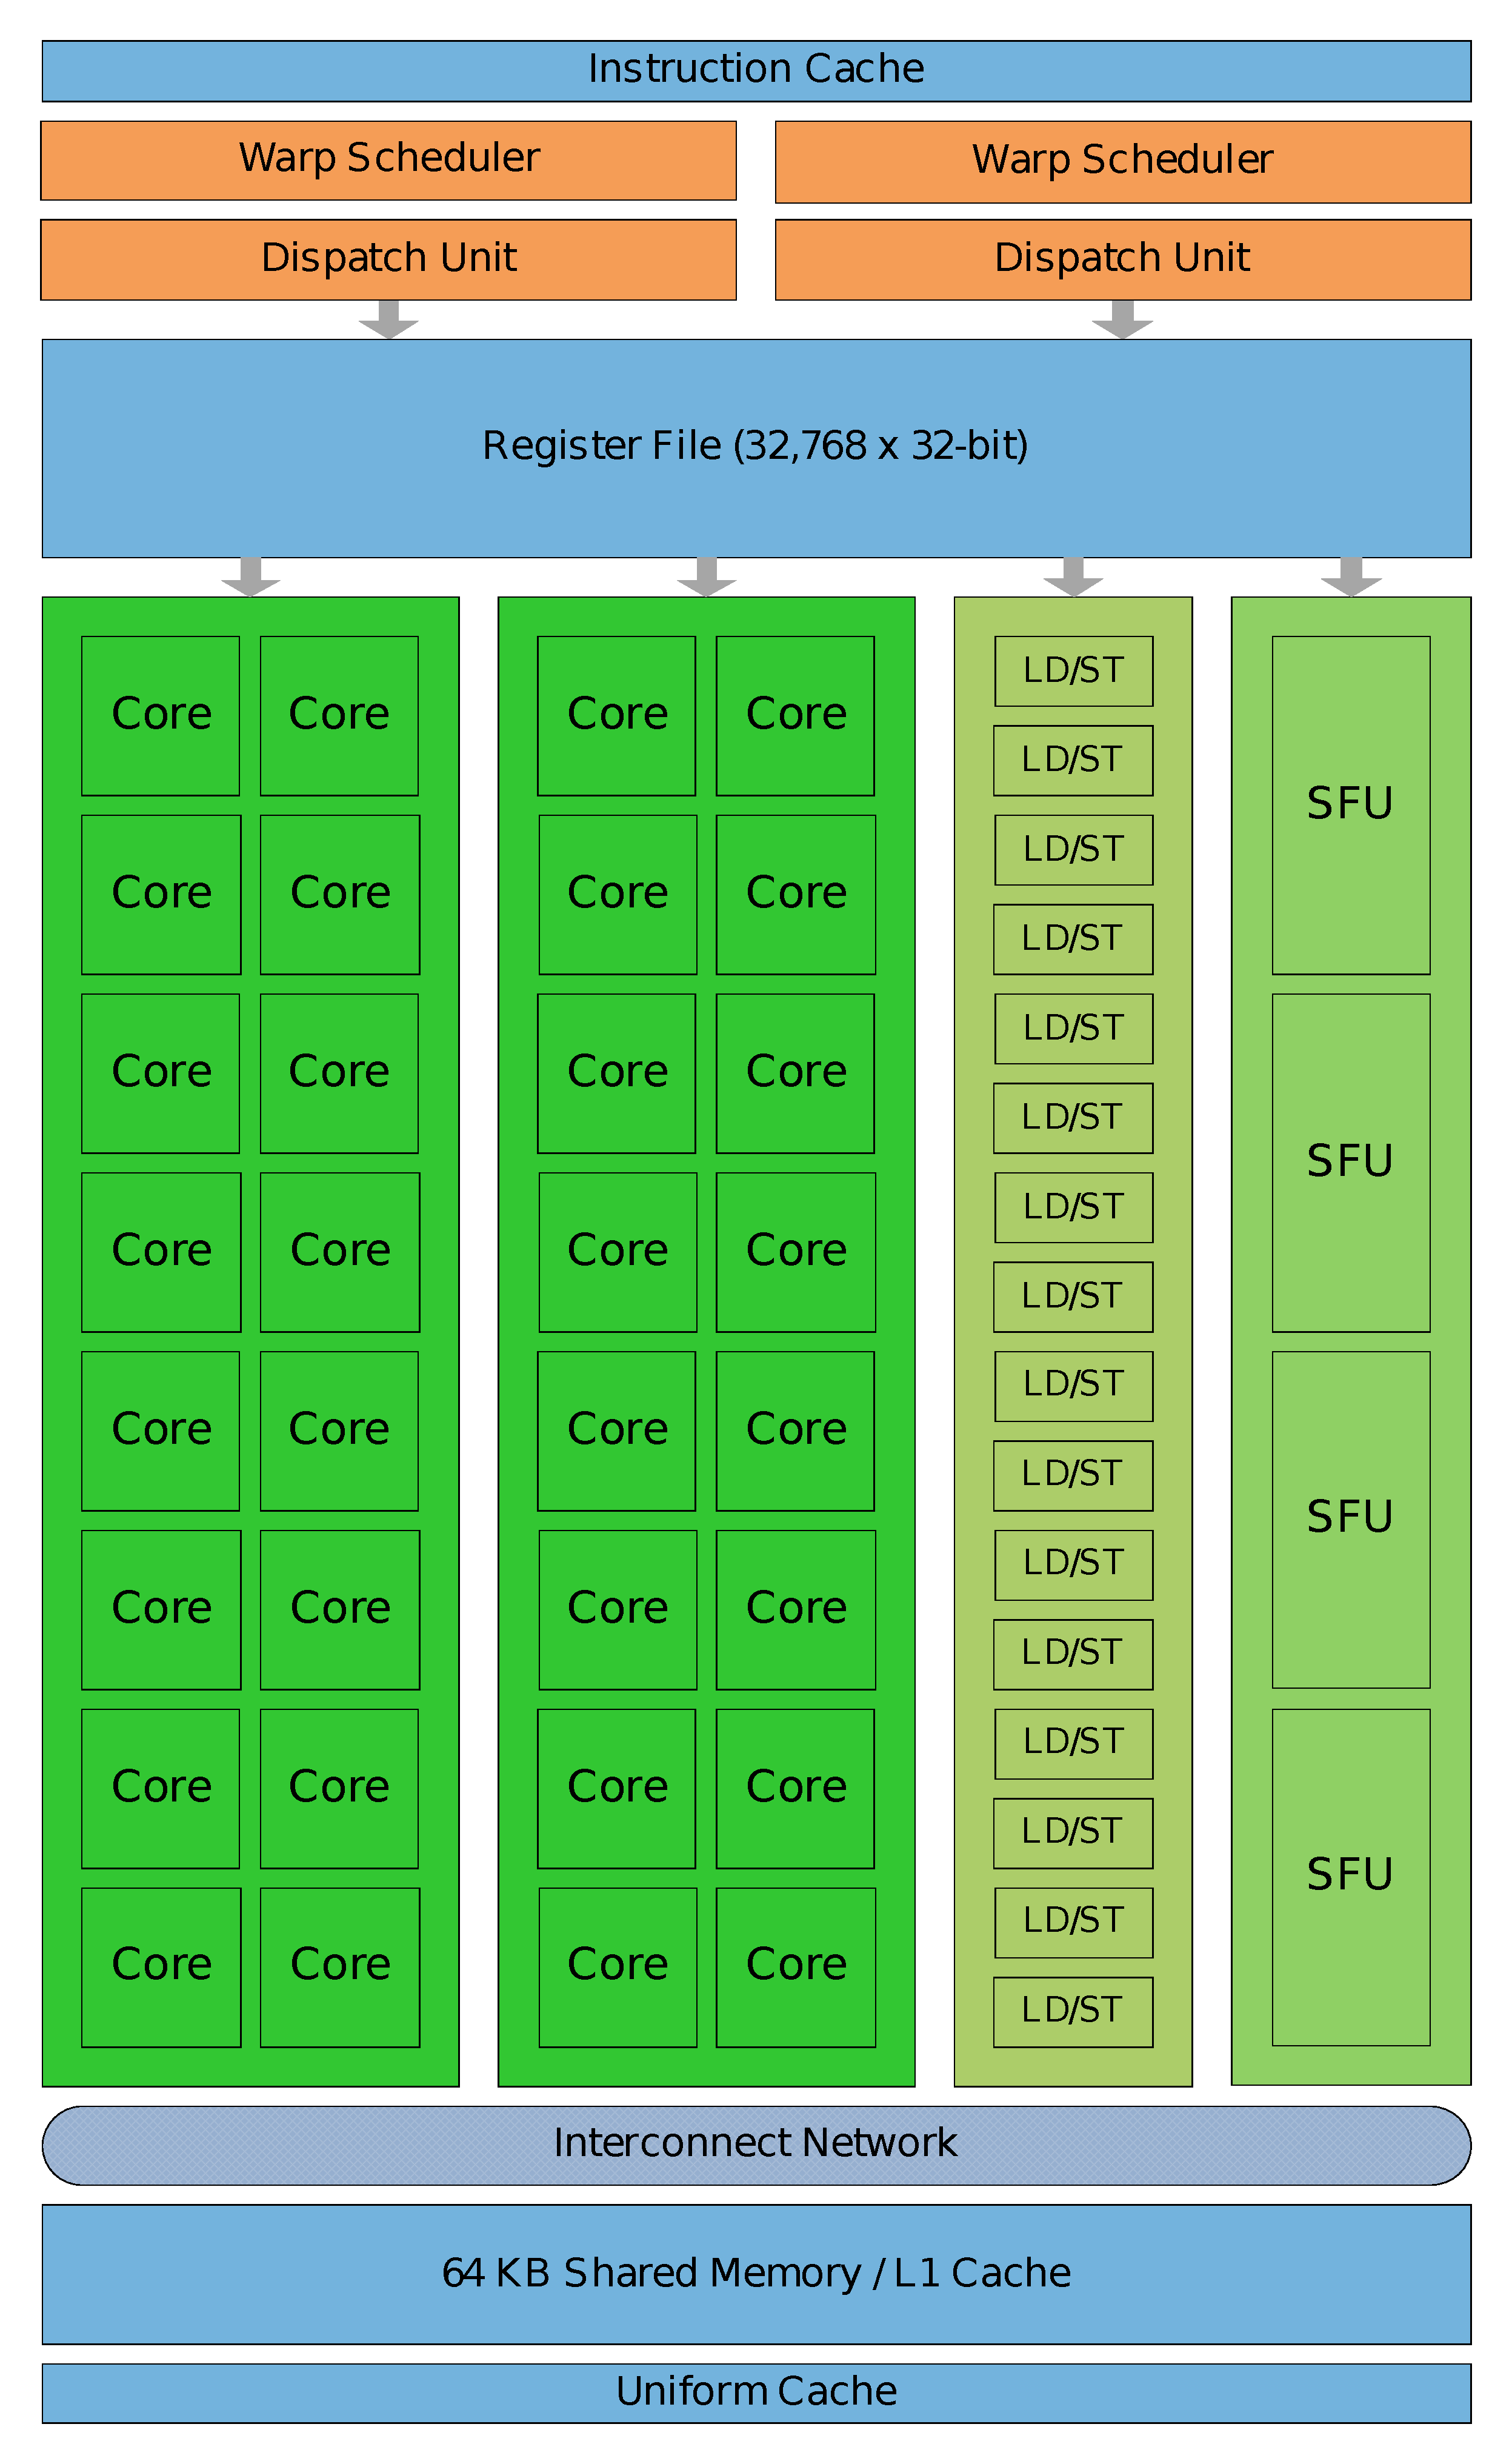
\includegraphics[width=\textwidth]{images/fermi-sm.pdf}
    \caption{Diagrama de bloques del SM de GF100 Fermi. Tomado de~\cite{NvidiaFermi}}
    \label{fermi_gpu_block}
\end{figure}

Los SM son unidades completas de ejecucion. Estos tienen 32 SPs interconectados entre si, que operan sobre
un register file com\'un a todos ellos. Los SM cuentan adicionalmente con multiples unidades de Load/Store,
que permiten realizar accesos a memoria independientes. Existen 4 unidades de SFU (\textit{Special Function
Unit}) por SM, para realizar rapidamente operaciones matematicas trascendentales (trigonometricas, potencias,
raices, etc.). Cada SM ejecuta simultaneamente una cantidad fija de threads, llamado \textit{warp}
con cada thread corriendo en un SP. Las unidades de envios de warps se encargan de mantener registro de que
threads estan disponibles para correr en un momento dado y permiten realizar cambios de contexto por hardware
muy eficientemente (alrededor 20-25 $\mu$segundos ~\cite{PattersonFermi}). Con esto, pueden ejecutar
concurrentemente dos warps distintos para esconder la latencia de las operaciones. En precision doble,
esto no se puede, asi que hay solamente un warp corriendo a la vez.

Un SM cuenta con una memoria com\'un de 64kb que se puede usar de forma autom\'atica tanto como memoria
compartida com\'un a todos los threads como cach\'e L1 para todos los accesos a memoria.

\begin{figure}[htbp]
    \centering
    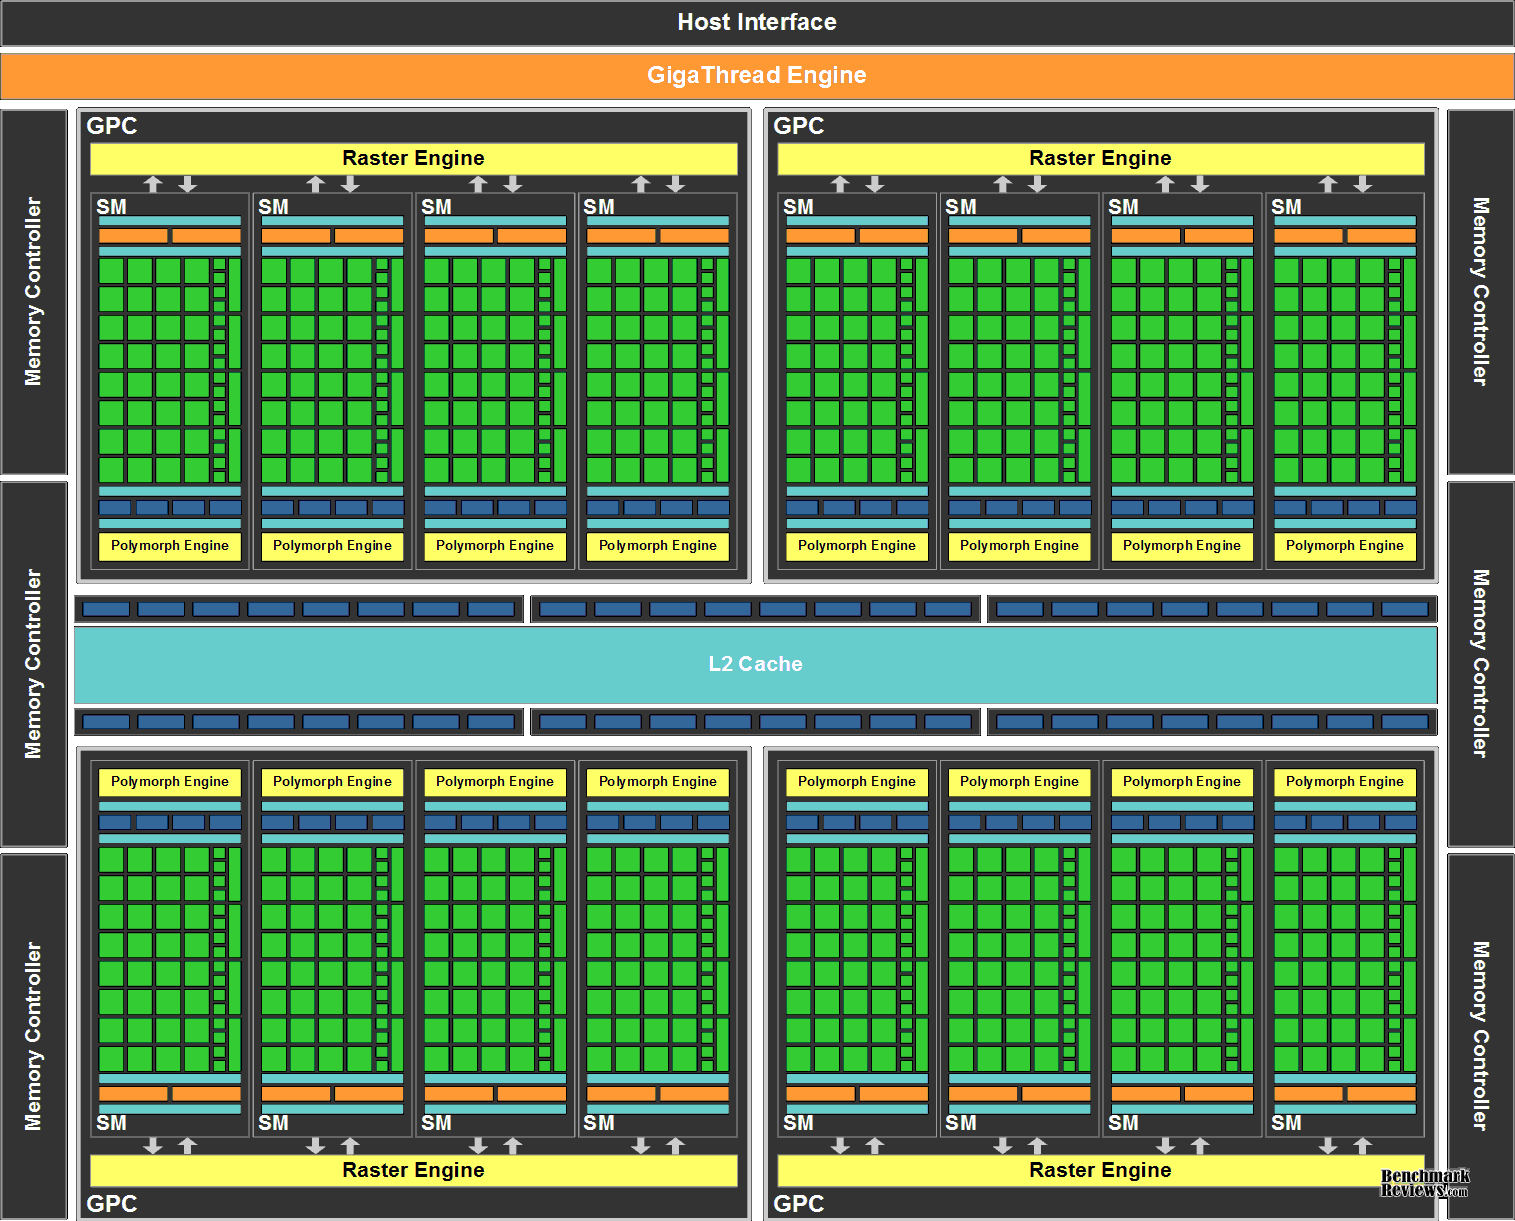
\includegraphics[width=\textwidth]{images/fermi-gpu-block.png}
    \caption{Diagrama de bloques de GF100 Fermi. Tomado de~\cite{NvidiaFermi}}
    \label{fermi_gpu_block}
\end{figure}


Por motivos de como funciona un pipeline grafico, los SM se agrupan de 4, en un GPC (\textit{Graphics
Processing Cluster}). Cada GPC se encarga de ejecutar los distintos pasos del pipeline gr\'afico,
cargando a los SM con las tareas que tienen que realizar para rasterizar (es decir, convertir los
gr\'aficos vectorialmente definidos en gr\'aficos renderizados). En aplicaciones de CUDA, estos pasos
no importan, puesto que se trata cada SM independientemente por software.

Todos los accesos a memoria global (la memoria off-chip del dispositivo) se realizan a traves de la memoria
L1 de cada SM, y a traves de la L2 del todo el procesador. Esta L2 consiste de 6 bancos de 128Kb, compartidas.
Estas cach\'e son write-through y se comunican de manera directa tanto con la DRAM propia de la placa como
con el bus PCI Express por el cual pueden comunicarse dos placas entre si, sin pasar por CPU.

En Fermi no se pueden ejecutar simultaneamente instrucciones de precision doble y simple, y como
las de doble requerien ambos pipelines, suelen disminuir considerablemente el aprovechamiento
de los cores. En Kepler, al usar 4 unidades de despacho de warp, puede elegir una mejor
combinaci\'on para poder ejecutar simultaneamente instrucciones que no dependan de las mismas
unidades funcionales en el pipeline. ~\cite{NvidiaKepler}

Como estos procesadores implementan el estandar IEEE754-2008, cuentan con precision simple y
doble correcta, por lo cual dentro de las operaciones nativas, cuentan con instrucciones FMA
(Fused multiply-add) que no pierden precisci\'on en etapas intermedias de redondeo.



%El c\'odigo escrito para CUDA se puede compilar a dos targets distintos; uno es
%el codigo binario nativo de la placa target donde se va a correr y el otro es un
%codigo intermedio, llamado c\'odigo PTX, que se JIT compila por el driver CUDA
%antes de enviar a la placa, de modo que sea portable entre placas y arquitecturas
%(retrocompatibles).

%Cuando se lanza un kernel de ejecuci\'on, este c\'odigo binario se carga en la DRAM propia
%de la placa. Este codigo va a ser ejecutado por todos los bloques que se hayan definido cuando
%se lanz\'o el kernel. El ``Thread Engine'' del GPGPU se encarga de repartir los bloques a los
%SM (Streaming Multiprocessors). Cada SM luego va a ejecutar de a grupos de 32 threads, cada uno
%de ellos corriendo sobre un SP (Streaming Processor). A traves de sus 2 o 4 unidades de dispatch de warp
%(de acuerdo a la generaci\'on de los chips), el SM puede dinamicamente cambiar el warp que se esta ejecutando en sus SP,
%escondiendo la latencia de los stalls de pipelines forzosos para la ejecucion de instrucciones de multiples clocks.
%Estos threads a su vez obtienen sus registros de un register file com\'un a todos los SP. Un scoreboard
%es mantenido por cada dispatcher de warps para poder determinar que threads estan listos para correr. En Kepler
%este scoreboard es simplificado ya que las latencias de las operaciones matem\'aticas es conocido, por
%lo cual se puede reemplazar por contadores m\'as sencillos. ~\cite{NvidiaKepler}
%Como el c\'odigo se ejecuta de manera sincr\'onica entre todos los threads del warp, las instrucciones
%condicionales proveen un problema para esta arquitectura. Como las distintas ramas del condicional
%son instrucciones excluyentes, no las deben ejecutar todos los threads simultaneamentes. El procesador
%deshabilitaba los cores que manejaban los threads de las ramas que no se ejecutaban del
%condicional~\cite{NvidiaTesla}. Para disminuir la cantidad de instrucciones de condicionales
%que se ejecutan, se cuenta con ~\cite{NvidiaFermi} predicaci\'on en todas las instrucciones de la ISA.


\subsubsection{Organizacion de la memoria}

%La arquitectura CUDA esta enfocada a procesamiento de grandes cantidades de datos
%de puntos flotante. El procesador GPGPU cuenta con cientos de ALU sincronizadas
%por bloques, permitiendo un paralelismo adaptativo a distintos problemas.
%
%El procesamiento GPGPU es similar al procesamiento vectorial
%realizado por las supercomputadoras Cray y IBM que surgio en los 1960's, pero
%en vez de usar VLIW para procesamiento masivo, CUDA usa multiples hilos de ejecuci\'on
%que trabajan simultaneamente sobre los datos.
%El procesamiento consiste en un funcionamiento hibrido entre compilador y procesador. Se determina
%un conjunto de elementos a procesar y se elije de manera explicita una manera de particionar el
%problema a la hora de ser enviado para procesado a la placa.
%
%Para realizar el computo, esta arquitectura cuenta a su vez con multiples clases de memorias
%que se adaptan de maneras diferentes a los distintos procesos. Estas incluyen:
La memoria de la GPGPU es uno de los puntos cruciales de esta arquitectura. Esta se subdivide
entre memorias on-chip y memorias off-chip, de acuerdo a su locacion y tiempos de acceso.

Las memorias se subdividen en 4 categorias distintas:

\begin{itemize}
  \item Registros
  \item Memoria global
  \item Memoria local
  \item Memoria compartida
\end{itemize}

Los registros son la unidad basica de almacenamiento de los threads de ejecuci\'on.
Cada thread de ejecuci\'on cuenta con una cantidad limitada de registros de punto flotante de
32 bits con latencia de un par de ciclos de clock. A su vez, existen una cantidad finita de
registros totales que cuenta un chip (oscilan entre 16.535 y 65.535 registros).

La memoria global es la memoria principal fuera del chip del GPGPU. Esta es de gran tama\~no (de
entre 2Gb y 12Gb) y es compartida por todos los SM de la GPGPU y los CPU que integran el
sistema. Es decir, tanto los GPGPU y los CPU pueden invocar las funciones del driver CUDA
para poder transferir datos entre la placa y la memoria RAM. La latencia de acceso a la memoria global
es de cientos de ciclos, sumamente lenta en comparaci\'on con el procesador.

La memoria compartida, o \texttt{shared} es una memoria que es visible para todos los threads dentro
de un mismo SM .Cada thread puede escribir en cualquier parte de la memoria compartida de su bloque y
puede ser leido por cualquier otro thread de su bloque. Es una memoria muy r\'apida, on-chip, y
que tarda una peque\~na cantidad de ciclos de acceso. Esta memoria es compartida con la cach\'e
nivel 1, de capacidad de entre 16Kb y 64kb configurable por software.

La memoria local es una memoria local a cada thread, que se encuentra almacenada dentro de la
memoria global. Esta memoria es definida automaticamente por el compilador y sirve como area de spilling
de registros cuando se acaban. Cuenta con las mismas desventajas que la memoria global, incluyendo
su tiempo de acceso.

Adicionalmente, la GPGPU cuenta con multiples niveles de memorias cach\'e para poder aminorar el hecho
de que el principal cuello de botella del computo es la latencia en los accesos a memoria global.
Estas se dividen en tres:

\begin{itemize}
  \item Cach\'e L1
  \item Cach\'e L2
  \item Cach\'e de textura
\end{itemize}

La cach\'e L1 es dedicada por SM. Esta cach\'e fue introducida en Fermi y su dise\~no hace que
tambien esta dedicada a la memoria compartida, por lo que es posible en tiempo de ejecuci\'on
darle directivas a la GPGPU que asigne m\'as memoria cach\'e o m\'as memoria compartida,
permitiendo a los bloques tener mayores espacios de memorias compartidas o mayores hit rate de cach\'es.

La cach\'e L2 es com\'un a todos los SM de la GPGPU, donde, a partir de Fermi en NVIDIA, todos
los accesos de lectura y escritura a memoria global y textura pasan a traves de esta. ~\cite{NvidiaFermi}

La cach\'e de textura es una cach\'e sobre la memoria global que presenta no solo localidad espacial,
como la mayoria de las cach\'es de procesadores normales (i.e. dato-1, dato, dato+1, etc.), sino que se le
puede agregar el concepto de dimensiones, para poder modelar datos en mas de una dimension.
Esto se adapta de muy bien a los problemas de gr\'aficos en el 2D y 3D, por lo tanto se convierte
en una herramienta clave a la hora de minimizar los accesos a matrices
no solo por filas sino por columnas. Esta cach\'e se debe definir en momento de compilaci\'on en
en el c\'odigo, ya que tiene limites espaciales (necesarios para poder definir areas de memoria
sobre la cual operar) y a su vez se debe acceder a los datos subyacentes a traves de funciones especificas. Una caracteristica adicional
de esta cach\'e es que como necesita resolver estos accesos no convencionales a la memoria, cuenta
con una unidad propia de resoluci\'on de direcciones. Esta unidad tiene limitantes a cuanto podemos
exigirle, ya que no posee un ancho de banda suficiente como para resolver todos los
accesos a memoria globales podria servir, asi que hay que usarla judiciosamente.


\subsubsection{Esquema de paralelismo}
El paralelismo en CUDA principalmente se divide en varios niveles:
\begin{itemize}
  \item Bloques de threads
  \item Grilla de bloques
  \item Streams
  \item Multiples placas
\end{itemize}

El paralelismo a nivel de bloque instancia una cantidad de threads, subdivididos logicamente en 1D, 2D o 3D.
Los threads internamente se agrupan de a 32 threads (un \textit{warp}).
Cada uno de estos threads va a contar su propio threadId y con el mismo blockId, identificandolos univocamente.
Estos threads van a correr simultaneamente en el mismo SM y van a ser puestos y sacados de ejecuci\'on
dinamicamente por el scheduler de hardware que cuenta la GPU. Para compartir informaci\'on entre
ellos, se puede utilizar la memoria shared o las instrucciones de comunicacion de threads intrawarp.

El paralelismo a nivel de grid determina una matriz de bloques de ejecuci\'on que particiona
el dominio del problema. El GigaThread Scheduler va a poner a ejecutar cada bloque en un SM hasta
el final de la ejecuci\'on de todos los threads. Los bloques entre si no comparten informaci\'on
sino a traves de la memoria global. Como no se garantiza ningun orden de ejecucion no se puede
confiar en sincronizar entre si.

El paralelismo de stream es una herramienta empleada para hacer trabajo multithreaded usando una
sola placa. Esta t\'ecnica permite que multiples threads encolen kerneles o copias de memoria
independientes, para que el driver pueda schedulearlas simultaneamente si se estan subutilizando
los recursos. Los streams permiten kernels concurrentes pero cuentan con importantes restricciones
que generan sincronizaci\'on implicita, lo cual hay que tener presente si se desea mantener el trabajo
de forma paralela.

El paralelismo a nivel de placa consiste en poder distribuir la carga del problema entre distintas
GPGPU dispuestas en un mismo sistema compartiendo una memoria RAM com\'un como si fuera un software
multithreaded tradicional. CUDA no cuenta con un modelo implicito de paralelismo entre distintas placas,
pero es posible hacerlo manualmente eligiendo de manera explicita que dispositivo usar. Las placas
se pueden comunicar asincronamente entre si, tanto accediendo a las memorias globales de cada una
como ejecutando c\'odigo remotamente. En las versiones modernas del driver de CUDA, tambien pueden
directamente comunicarse las placas entre si a traves de la red, permitiendo escalar multinodo facilmente.

Un algoritmo en GPGPU debe considerar todos estos niveles de paralelismo para poder maximizar la
performance empleando todos los recurosos con los que cuentan estos dispositivos.

\subsubsection{Diferencias entre Tesla, Fermi, Kepler}

Hasta ahora enunciamos la arquitectura vista desde el punto de vista Fermi, la segunda
arquitectura dise\~nada por Nvidia que era GPGPU. Fermi es la evoluci\'on de Tesla,
construida para desacoplar a\'un mas los conceptos de gr\'aficos de modo de hacerla
un procesador m\'as escalable y de proposito general.

\begin{table}[h]
\caption{Tabla comparativa de las features mas prominentes de las tres arquitecturas de CUDA}
\label{tab:CudaGenerations}
\begin{tabular}{lllll}
                 & Tesla (GT200) & Fermi (GF100) & Kepler (GK110) &  \\
A\~no            &               &               &                &  \\
SMs              &               &               &                &  \\
Cores/SM         &               &               &                &  \\
Cache L1         &               &               &                &  \\
Cache L2         &               &               &                &  \\
Registros/Thread &               &               &                &  \\
Tecnologia de fabricaci\'on &    &               &                &  \\
                 &               &               &                &  \\
                 &               &               &                &
\end{tabular}
\end{table}

En la tabla \ref{tab:CudaGenerations} vemos una comparaci\'on de las recursos que estan m\'as directamente
relacionadas a la performance de un c\'odigo en GPGPU. En esta podemos apreciar como muchos recursos
aumentaron drasticamente gracias a las tecnologias de fabricaci\'on, que permitieron aumentar la
cantidad de transistores. Tambien podemos comprobar que, a diferencia de los CPU, las arquitecturas GPGPU
decidieron utilizar esos nuevos transistores disponibles para mas nucleos de procesamiento, en vez
de dedicarlas a aumentar las memorias cach\'e, que crecieron minimamente.


\subsubsection{CUDA, Herramientas de desarrollo, profiling, exploracion}

Para soportar una arquitectura masivamente paralela, se debe usar una ISA
(\texttt{Instruction Set Architecture}) dise\~nada especialmente para el problema. Esta ISA, conocida como PTX,
debe poder soportar conceptos fundamentales del computo GPGPU: grandes cantidades de registros,
operaciones en punto flotante de precision simple y doble y fused multiply-add. Adem\'as,
el c\'odigo compilado para GPGPU debe ser agn\'ostico al dispositivo que lo va a correr, por
lo cual la paralelizaci\'on no debe estar demasiado atada a este, sino que el dispatching
lo debe poder determinar el driver de la placa en tiempo de ejecuci\'on. De este modo, la paralelizaci\'on
deberia ser la m\'as apropiada en cada dispositivo, sin importar la generaci\'on que sea. Un \'ultimo
requerimiento clave de esta ISA es que debe poder soportar poder realizar ajustes manuales,
para poder construir partes claves de ciertas librerias frecuentemente usadas (como las BLAS)~\cite{NvidiaFermi}.

El lenguaje que desarrollo Nvidia para poder programar estos dispositivos a un nivel m\'as alto
que el assembler especifico de la placa es CUDA. Este lenguaje es una extension de C++, con ciertas
features agregadas para poder expresar la subdivision de los kernels en threads y bloques.
Este c\'odigo se compila usando el \texttt{nvcc}, una variante del \texttt{GNU gcc} que se
encarga de generar el c\'odigo PTX para las funciones marcadas como que se van a ejecutar
en los dispositivos. Esto despues se linkea normalmente y se genera un binario ejecutable.

Nvidia, ademas, provee herramientas de profiling para explorar como se estan utilizando los
recursos durante la ejecuci\'on. Estas son imprescindibles para optimizar, puesto que los limitantes
de GPU son sumamente distintos a los de CPU, presentando dificultades incluso para programadores
experimentados. Las herramientas de profiling no solo muestran runtime, sino que sirven para
ver donde hay accesos a memoria excesivos, puntos de sincronizaci\'on costosos, limitantes
en los registros.


\subsubsection{Requerimientos de un problema para GPGPU}
En un principio, al ser GPGPU una arquitectura con completo poder expresivo, se puede
calcular cualquier cosa. Sin embargo, hay altos costos en los que se incurren antes de
poder ejecutar c\'odigo. Un problema debe exhibir al menos las siguientes caracteristicas
para que valga la pena poder pensar en correrlo para GPGPU.
\begin{enumerate}
  \item \label{req:paralelo} El problema debe tener una gran parte paralelizable.
  \item \label{req:float} El problema debe consistir mayormente de operaciones numericas de punto flotante.
  \item \label{req:matrix} El problema debe poder ser modelado mayormente en arreglos o matrices.
  \item \label{req:transf} El tiempo de computo debe ser muy superior al tiempo de transferencia de datos.
\end{enumerate}

Item \ref{req:paralelo} se refiere a que debe existir alguna forma de partir el problema
en subproblemas que puedan realizarse simultaneamente, sin que haya dependencias de
resultados entre si. Si el problema requere partes seriales, lo ideal es que se las
pueda concebir las partes paralelas sean etapas de un pipeline de procesos, donde
cada una de estas exhiban caracteristicas fuertemente paralelas. Como las arquitecturas
masivamente paralelas tienen como desventaja una menor eficiencia por core, si el
problema no se puede dividir para maximizar la ocupancion de todos los cores disponibles,
va a ser muy dificil superar en eficiencia a los procesadores seriales.

Item \ref{req:float} habla de que el m\'etodo de resoluci\'on de los problemas debe
consistir del uso de m\'etodos numericos. El set de instrucciones de las arquitecturas
de GPGPU estan fuertemente influenciados por las aplicaciones 3D que las impulsaron
en un principio. Estas consisten mayormente de transformaciones de \'algebra lineal
para modelar luces, hacer renders o mover puntos de vistas. Todos estos problemas
son inherentemente de punto flotante, por lo cual el set de instrucciones, las ALUs
internas y los registros estan optimizados para este caso de uso. Las operaciones
en numeros enteros no son el fuerte de esta arquitectura y suelen ser realizados
m\'as eficientemente por procesadores de proposito general.

Item \ref{req:matrix} menciona que los problemas que mejor se pueden tratar en esta
arquitectura se pueden representar como operaciones entre arreglos o matrices de
dos, tres o cuatro dimensiones. Las estructuras de datos que no estan secuenciales
en memoria pueden incurrir en multiples accesos a esta para recorrerlas, y en las
arquitecturas GPGPU son estos los que generan el mayor cuello de botella. Ademas,
suelen ser dificiles de paralelizar en m\'ultiples subproblemas. Tener como parametros de
entrada matrices o arreglos que se puedan partir facilmente incurre en minimos
overheads de computo y permite aprovechar mejor las memorias caches y las herramientas de
prefetching que brinda la arquitectura.

Item \ref{req:transf} ataca uno de los puntos criticos de esta arquitectura. Para poder
operar con datos, se requiere que estos esten en la memoria de la placa, no la memoria
de proposito general de la computadora. Esto quiere decir, que se deben hacer copias
explicitas entre las memorias, ya que ambas tienen espacios de direcciones independentientes.
Esta copia se realiza a traves de buses que, a pesar de tener un enorme throughput de
datos, tambien tienen una gran latencia (orden de milisegundos). Por lo tanto, para minimizar
el tiempo de ejecuci\'on de un programa usando las GPGPU, se debe considerar tambien el
tiempo de transferencia de datos a la hora de determinar si el beneficio de computar en
menor tiempo lo justifica. Las nuevas versiones de CUDA buscan brindar nuevas herramientas
para simplificar este requerimiento, proveyendo espacio de direccionamiento unico \ref{CUDA4} y
memoria unificada \ref{CUDA6}, pero siguen siendo copias de memoria a traves de los
buses (aunque asincronicas).

Estas caracteristicas limitan enormemente la clase de problemas que una GPGPU puede
afrontar, y suelen ser una buena heuristica para determinar de antemano si vale la pena
invertir el tiempo necesario de la implementaci\'ony ajuste fino.


\subsubsection{Diferencia entre CPU y GPU - Procesadores especulativos}
Viendo la historia de CPU, podemos hacer un recorrido de los problemas que los dise\~nadores de procesadores
fueron enfrentandose a lo largo del tiempo mirando los componentes que fueron apareciendo.

(insertar foto de die de nehalem)

Caches - Pipelines - Predictores - M\'as cach\'e - M\'as controladores de memoria - Multiple issues

Lo importante ac\'a es observar el patron: ``no desechar algo que podramos necesitar pronto'',
``intentar predecir el futuro de los condicionales'', ``intentar correr multiples instrucciones a la vez
porque puede llegar a bloquear en alguna de ellas.''

Todos estos problemas convierten al CPU en una maquina que gira alrededor de la especulacion,
de los valores futuros que van a tener las ejecuciones, del probable reuso de datos.
Podemos observar entonces que las unidades que verdaderamente hacen la ejecuci\'on de las operaciones,
las ALU, son muy pocas en comparaci\'oncon la cantidad de dispositivos de soporte que estan
sobre el die del CPU.

En contraste, las arquitecturas GPGPU son verdaderas maquinas de computo masivo. Estan dise\~nadas para
resolver una y otra vez operaciones muy bien definidas (intrucciones de punto flotante en su mayoria).
Comparativamente con un CPU, las ALU de las GPU son bastante pobres y lentas. No funcionan a las mismas
velocidades de clock y deben estar sincronizadas entre si. Pero la gran ventaja esta en la cantidad.
Un CPU cuenta con unas pocas ALU por core, dependiendo de su algoritmo de scheduling interno
(alrededor de 16 cores por die de x86 es el tope de linea ofrecido actualmente). Un GPU cuenta con miles de ALUs en total
(m\'as de 2500 CUDA Cores en Tesla K20). Un GPU, en cambio, dispone de pocas unidades de soporte del procesamiento.
No cuenta con pipelines especulativos, el tama\~no de las caches
estan a ordenes de magnitud de las de CPU, la latencia a las memorias principales de la GPU estan a
decenas de clocks de distancia, etc. La arquitectura asume que siempre va a tener m\'as trabajo
para hacer, por lo cual en vez de intentar solucionar los pitfalls de un grupo de threads, directamente
los reschedulea para m\'as adelante y continua procesando otro warp de threads. Se puede notar que durante del
dise\~no de la arquitectura GPGPU buscaron resolver el problema del computo masivo pensando en hacer
m\'as cuentas a la vez y recalcular datos viejos de ser necesario. Esto es una marcada diferencia contra
los CPU, que estan pensado en rehacer el menor trabajo posible y intentar mantener todos los datos que pueda en
las memorias caches gigantescas.

Como los CPU tienen que poder soportar cualquier aplicacion, no pueden avocarse de lleno a una sola
problematica. El hecho de no tener que dise\~nar un procesador de proposito general permitio un cambio radical
a la hora de pensar como concebir una arquitectura de gran throughput auxiliar al procesador, no reemplazandolo
sino mas bien adicionando poder de computo.~\cite{GlaskowskyFermi}

Las arquitecturas Fermi (y agregar AMD) han concebido el dise\~no de un procesador de alto desempe\~no.
Su meta principal es poder soportar grandes cantidades de paralelismo, mediante el uso de procesadores
simetricos, pero tomando la fuerte restricci\'on de ``no siempre tiene que andar bien''. Es decir, ellos
mismos asumen que el codigo que van a correr esta bien adaptado a la arquitectura y no disponen
casi de mecanismos para dar optimizaciones post-compilacion. Relajar esta restricci\'on
les permitio romper con el modelo de computo de CPU y definir nuevas estrategias de paralelismo,
que no siempre se adaptan bien a todos los problemas, pero para el subconjunto de los desafios que se
presentan en el area de HPC y de videojuegos han probado ser un cambio paradigm\'atico.

\subsubsection{Idoneidad para el problema}
El problema de QM/MM enfrentado en este trabajo cuenta con mutiples operaciones matematicas de gran
volumen de calculos. En particular, las operaciones matriciales son los cuellos de botella en este
problema.
Para obtener los valores numericos de densidad buscados en los puntos, se deben obtener las derivadas primeras
y segundas, lo cual implica hacer multiples operaciones de multiplicaci\'onmatricial. Estas multiplicaciones
pueden ser paralelizadas por columnas y por filas. Estos problemas estan fuertemente estudiados como paralelizarlos
en la literatura, ya que los problemas de algebra lineal los requieren constantemente.
En nuestro caso, se requieren para un sistema cientas de estas multiplicaciones, algunas con matrices de mas de
$500^2$ elementos. Al consistir este proyecto un sistema de resoluci\'on num\'erico de las f\'ormulas de QM/MM,
los problemas enfrentados eran casi en su totalidad de operaciones de punto flotante. Luego, dados las
caracteristicas de contar con un fuerte nivel de paralelismo en los cuellos de botella y de ser operaciones
mayormente de punto flotante, determinamos que el uso de las GPGPU era idoneo, en comparaci\'on con arquitecturas
de proposito general con menos GFLOPS.


\section {CPU}

\subsection{Introducci\'on}

Los microprocesadores ganan en prevalencia desde principios de los 70,
cuando Intel introduce los modelos 4004 y 8008. Actualmente las arquitecturas
de procesadores de 64 bits basadas en la l\'inea x86-64 de Intel
dominan no solo el mercado de computadoras personales sino que tambi\'en el de
servidores y \textit{clusters} de c\'omputo. Dado que utilizaremos el CPU
est\'andar como punto de comparaci\'on para las dem\'as arquitecturas, y que estas
est\'an basadas en parte en su dise\~no, daremos una breve rese\~na de los aspectos
m\'as importantes y desarrollos modernos con respecto a la performance dentro de
los procesadores modernos.

\subsection{Tipos de paralelismo}

Existen tres categor\'ias de paralelismo que una arquitectura puede aprovechar
para mejorar la \textit{performance} de una aplicaci\'on, ganando prevalencia
en el \'ultimo tiempo en el dise\~no de procesadores.

\begin{itemize}
    \item \textit{Instruction Level Parallelism}: Este tipo de optimizaciones buscan
    ejecutar la mayor cantidad de instrucciones en un mismo hilo de ejecuci\'on simult\'aneamente.
    Optimizaciones de este estilo incluyen
    \textit{pipelines} de procesador para ejecutar m\'ultiples instrucciones de manera solapada,
    ejecuci\'on superescalar fuera de orden para ejecutar m\'ultiples instrucciones que
    utilizan unidades del procesador distintas o que no dependen una de la otra, ejecuci\'on
    especulativa (basada en predicci\'on de resultados todav\'ia no finalizados de procesar), etc.

    \item \textit{Data Level Parallelism}: Consideran las optimizaciones cuyo prop\'osito es
    lograr aplicar una misma operaci\'on a cada elemento de un conjunto datos simult\'aneamente
    en un mismo hilo de ejecuci\'on. Esta t\'ecnica se denomina SIMD
    (\textit{Single Instruction, Multiple Data}).

    \item \textit{Thread Level Parallelism}: Concierne al uso de m\'ultiples hilos de ejecuci\'on
    simult\'aneos, lo cual requiere el uso de procesadores que usualmente
    comparten la memoria principal (arquitectura SMP, \textit{Symmetric Multiprocessing}).
    Esto conlleva esfuerzo adicional para mantener consistencia y coherencia de la misma
    para que no se convierta en un cuello de botella.
\end{itemize}

A continuaci\'on detallamos algunos aspectos de cada una de estas t\'ecnicas.

\subsection{Pipeline y Ejecuci\'on fuera de orden}

Los primeras implementaciones de paralelismo a nivel de un solo procesador fueron a nivel de instrucciones, mediante el uso
de \textit{pipelines} de m\'ltiples etapas. Estas llegaron a ser tantas como 20 distintas, en la arquitectura
Intel Pentium 4. Cada etapa corresponde a una actividad distinta en el proceso de ejecutar una instrucci\'on.
Al tiempo que una instrucci\'on es decodificada, por ejemplo, otra instrucci\'on puede estar siendo le\'ida
de memoria ya que, idealmente, las etapas previas no dependen de las posteriores. Este mecanismo funciona bien
si una instrucci\'on no depende de los resultados de otra que viene anterior a ella. Sin embargo, esto puede
ocurrir, produci\'endose entonces un \textit{pipe stall} que requiere ejecutar las instrucciones de manera no solapada
(con el costo de \textit{throughput} de instrucciones que ello implica).

Esta t\'ecnica llevada a su conclusi\'on l\'ogica se conoce como ejecuci\'on fuera de orden (\textit{Out of Order
Execution}). Mediante el uso de algoritmos y circuitos complejos, un procesador puede no depender del orden dado
de las instrucciones, sino solo de las dependencias entre las mismas, ejecutando etapas independientes para
instrucciones que no requieren datos entre si. De esta manera todas las unidades del procesador pueden estar
ocupadas el mayor tiempo posible.

Mejoras en este nivel eran usualmente invisibles al programador, dependiendo de los compiladores optimizantes,
pero sus ventajas fueron disminuyendo hacia principios del siglo XXI.

\subsection{Extensiones vectoriales}

Si bien las t\'ecnicas SIMD fueron desarrolladas por las supercomputadoras de los 70 y 80, su aparici\'on en los
microprocesadores x86 modernos ocurre en 1996 con el nombre MMX (\textit{MultiMedia eXtensions}), con refuerzos luego en las
extensiones SSE y AVX. AVX y AVX2 representan la \'ultima versi\'on de las instrucciones de vectorizaci\'on y est\'an presentes
en la l\'inea Intel Xeon de procesadores de alta gama y en las m\'as recientes generaciones de procesadores de consumidores.

El paralelismo de datos puede ser explotado por el compilador, que analiza los ciclos de programa y detecta cuando hay operaciones
independientes que pueden ser realizadas en simultaneo, dividiendo la cantidad de instrucciones totales que tiene que realizar
un procesador.

El uso de operaciones sobre m\'ultiples valores ha tomado importancia como uno de los m\'etodos de incrementar
la performance de ejecuci\'on. La longitud de registros SIMD de las extensiones (128 bits para SSE, 256 para AVX)
se ha duplicado cada 4 a\~nos, con lo cual es importante para una aplicaci\'on que sus operaciones sean lo m\'as
vectorizables posible.~\cite{HennessyPatterson} Para esto es ideal que las operaciones sean lo m\'as regulares y
los ciclos sean claros y con las m\'inimas dependencias posibles, de modo de hacer mejor uso de estas facilidades.

\subsection{Caches}

A diferencia de los procesadores, la velocidad de acceso de las memorias principales no aument\'o de una manera
tan significativa, como se puede ver en la figura~\ref{fig:cpu_vs_mem}. Como consecuencia, la memoria
empez\'o a convertirse en un serio cuello de botella a la velocidad de ejecuci\'on de los programas (llamado
en la jerga \textit{memory wall}).

\begin{figure}[htbp]
    \centering
    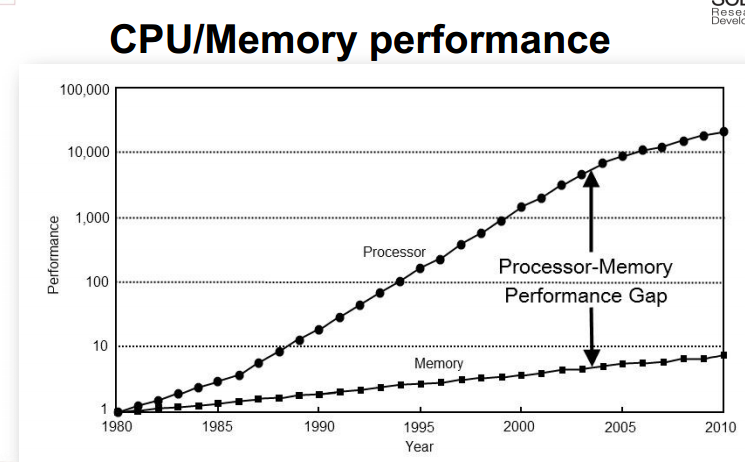
\includegraphics[width=\plotwidth]{images/cpu_vs_memory.png}
    \caption{Comaparaci\'on entre la \textit{performance} de CPU y memoria seg\'un el a\~no, mostrando
    el denominado \textit{memory gap}}
    \label{fig:cpu_vs_mem}
\end{figure}

Empleando el concepto de \textit{localidad}, producto de la observaci\'on de que los datos con los que opera una
secci\'on de un programa suelen estar cerca en memoria, los dise\~nos de procesadores empezaron a incluir distintos
tipos de caches: unas memorias r\'apidas, pr\'oximas al CPU y de menor tama\~no para contener el subconjunto de los datos
recientemente usados. Su eficacia impuls\'o el uso de una jerarqu\'ia de las mismas, organizadas en orden creciente
de tama\~no y decreciente en velocidad, empezando por las caches L1 y siguiendo por las L2 y L3.

El tama\~no de una cache L1 moderna est\'a en el orden de los 64 Kb, una cache L2 en el \'orden de los 2 Mb y
una L3 en el orden de 6 Mb en adelante.

Si bien idealmente la aparici\'on de caches es invisible al programador, y usualmente lo es, accesos irregulares a la
memoria pueden producir que la cache se cargue con datos que no volver\'an a ser utilizados, causando que datos posteriormente
a utilizar se hayan perdido y deban ser buscados nuevamente en la relativamente lenta memoria principal (evento que se conoce como
\textit{cache miss}). Por esto es que la regularidad de los accesos a memoria para hacer buen uso de caches es
fundamental cuando la performance es de importancia.

\subsection{Multiprocesadores}

Los procesadores MIMD (\textit{Multiple Instruction Multiple Data}) implicaron una revoluci\'on en la computaci\'on, pero
cada procesador continua las l\'ineas anteriores.  Los dise\~nos m\'as utilizados se basan en SMP (\textit{Symmetric
Multiprocessing}), donde todos los procesadores son iguales y comparten una misma memoria principal. Cada procesador tiene
sus propios registros y se comunica con los dem\'as mediante memoria compartida o interrupciones.

Por ejemplo, el procesador Intel Xeon E7-8800 posee 12 procesadores (cores) que pueden ejecutar dos hilos simult\'aneamente
cada uno, mediante el uso de tecnolog\'ias como \textit{Hyper-threading}.

A diferencia de los otros m\'etodos, las mejoras posibles mediante el procesamiento paralelo en tareas son sustanciales,
pero dependen grandemente del programador. Un programa serial no se beneficiar\'a de m\'ultiples \textit{cores},
incluso siendo recompilado, a menos que este paralelismo se aproveche expl\'icitamente. Otro aspecto importante es la
\textit{escalabilidad}, que consiste en que la divisi\'on de tareas mantenga a todos los procesadores disponibles ocupados,
aunque la cantidad de los mismos crezca.

Un resultado importante a tener en cuenta es la denominada \textit{Ley de Amdahl}, que establece una relaci\'on entre
el \textit{speedup} m\'aximo alcanzable mediante un incremento en la cantidad de procesadores disponibles, el porcentaje
de la aplicaci\'on que es paralelizable y el porcentaje que no lo es. Matem\'aticamente,

\begin{equation}
    \label{eq:amdahl}
    S(n) = \frac{1}{1 + \frac{1}{n} (1 - B)}
\end{equation}

Donde $S$ es el porcentaje m\'aximo de mejora alcanzable, $B$ es la fracci\'on del algoritmo a ejecutar que debe ejecutarse
serialmente, y $n$ la cantidad de hilos de ejecuci\'on paralelos que se dispone.

\begin{figure}[htbp]
    \centering
    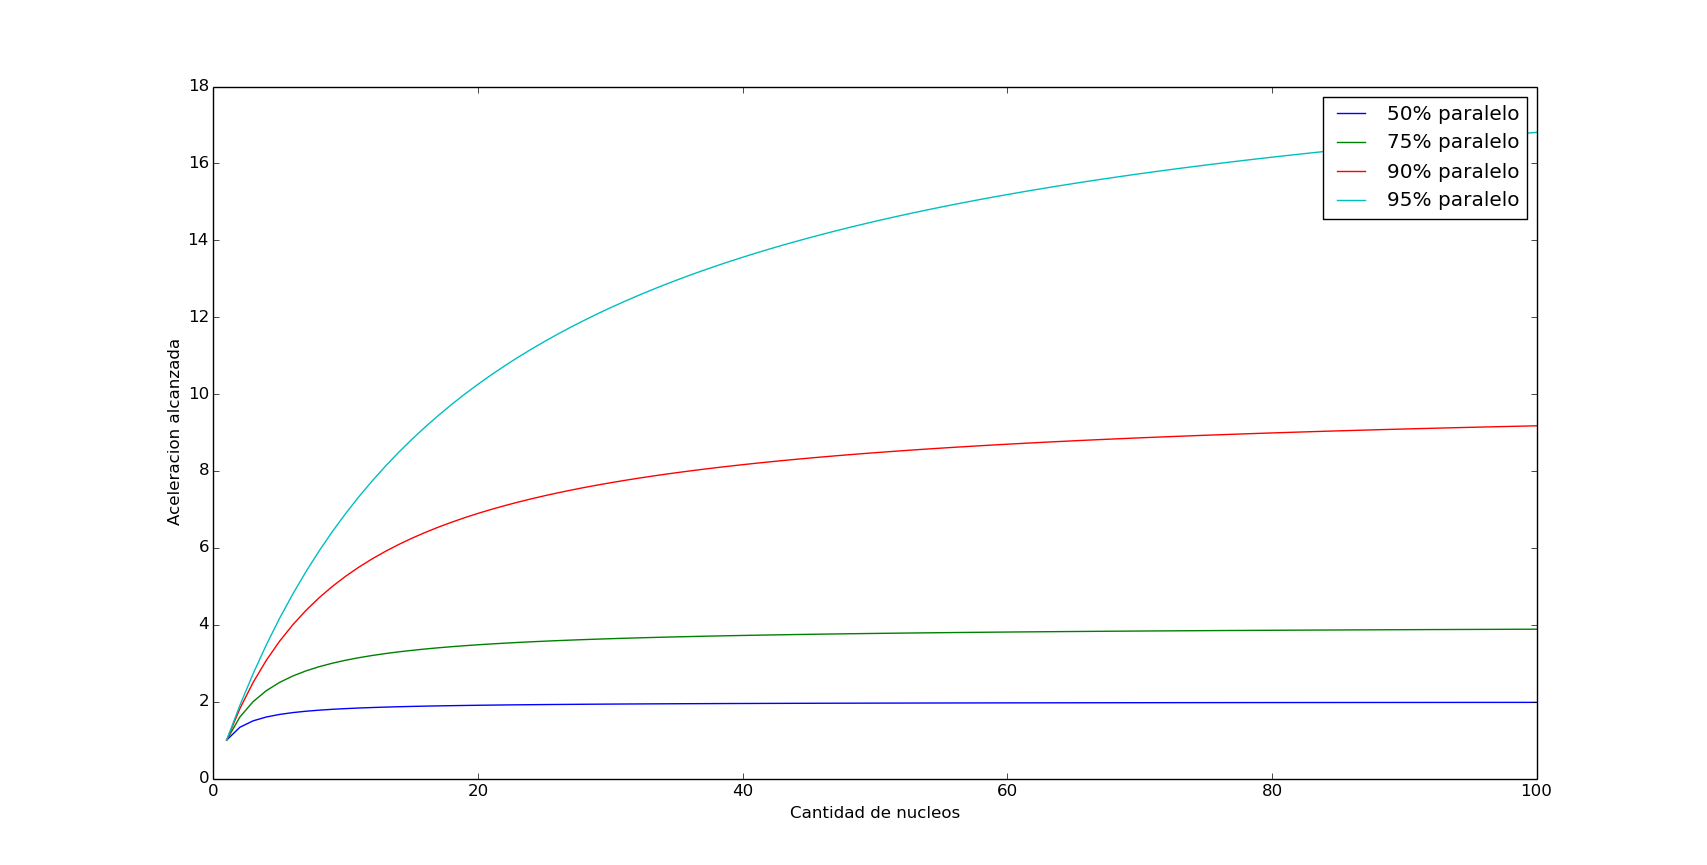
\includegraphics[width=\plotwidth]{plots/cpu/amdahl.png}
    \caption{Aceleraci\'on te\'orica m\'axima (en veces) dada por la ley de Amdahl, seg\'un la cantidad de n\'ucleos de procesamiento}
    \label{fig:amdahl_plot}
\end{figure}

Un ejemplo de esta ley en acci\'on es que si $95 \%$ del problema es paralelizable entonces el l\'imite te\'orico de
mejora es de 20 veces (el programa corriendo sobre infinitos cores se ejecutar\'ia en un veinteavo del tiempo que originalmente
requer\'ia). La figura ~\ref{fig:amdahl_plot} muestra el comportamiento de la ley de Amdahl con distintas fracciones de c\'odigo
paralelo.

La ley de Amdahl describe el pico te\'orico de mejora y es una simplificaci\'on, ya que asume que todos los cores tienen
trabajo perfectamente distribuido sin comunicaci\'on entre ellos por motivos de sincronizaci\'on.

Por otro lado, la presencia de un componente com\'un (la memoria) puede introducir cuellos de botella en el acceso a los
datos, ya que si el \textit{bus} de memoria es saturado con pedidos los procesadores deben detener su ejecuci\'on hasta que
los datos est\'en listos, elimin\'andose entonces el procesamiento paralelo.

Otro elemento de conflicto son los caches. Como los procesadores deben tener una visi\'on unificada y consistente de la
memoria, a veces es necesario que estos sincronicen los valores de sus caches, especialmente ante una escritura de memoria.
Esto se conoce como \textit{coherencia de caches} e involucra una sincronizaci\'on de alto \textit{overhead}, ya
que implica coordinaci\'on entre dos o m\'as procesadores a trav\'es de un bus de memoria.

Es en este punto que el impacto del paralelismo en el comportamiento del programa puede ser tan fuerte como sutil. Un fen\'omeno que
ilustra esto es el de \textit{false sharing}. Este fen\'omeno sucede cuando una variable no compartida entre threads
reside en la misma l\'inea de cache con una que si, requiriendo entonces que sea pasada de lado a lado entre cores aunque
nunca fuese esto necesario, decrementando la escalabilidad del algoritmo a muchos procesadores y siendo
dif\'icil de descubrir al depender intr\'insecamente del sistema en el que se corre.

\subsubsection{Hardware}

La arquitectura del Xeon Phi, parte de la linea de Intel Many Core Architecture (MIC), est\'a esquematizada
en la figura~\ref{fig:xeon_phi_arch}. Cada procesador esta esquematizado en~\ref{fig:xeon_phi_core}

La base de esta arquitectura consiste entre 60 y 80 cores SMP (\textit{Symmetric Multiprocessing}), con lo cual todos
ellos comparten la misma memoria principal. Cada uno de los cores tiene un \textit{clock rate} de 1 GHz,
con una arquitectura similar al set de instrucciones de Intel IA-32. Las principales diferencias con este
conjunto de instrucciones son el soporte para direccionamiento a 64 bits y nuevas instrucciones de vectorizaci\'on.

Cada procesador tiene adem\'as soporte para 4 \textit{threads}, es decir, 4 hilos de ejecuci\'on diferentes. Adicionalmente,
cada \textit{thread} puede ejecutar dos instrucciones por ciclo de clock, mediante el uso de dos pipes: \textit{V-pipe} y \textit{U-pipe}.
Algunas instrucciones, sin embargo, solo puede ser ejecutadas en una de las dos: por ejemplo las instrucciones de vectorizaci\'on solo pueden
ser ejecutadas en la \textit{U-pipe}. Para ejecutar estas instrucciones se dispone de una unidad de vectorizaci\'on (VPU, \textit{Vector Processing Unit}).
Esta unidad cuenta 32 registros SIMD (Single Instruction Multiple Data) de 512 bits. La latencia de estas instrucciones es de 4 ciclos de clock pero permiten
operar sobre 16 valores de punto flotante de precisi\'on simple (\textit{float}) a la vez.

Adem\'as de la unidad de vectorizaci\'on y la unidad escalar, cada procesador cuenta con 32 Kb de cache L1 y 512 Kb de cache
L2. Estas caches son asociativas \textit{8-way} y su linea de cache tiene 64 bytes. La coherencia de cach\'e se mantiene
mediante un directorio distribuido de \textit{tags} (v\'ease figura~\ref{fig:xeon_phi_arch}) dividido en 64 secciones e implementado
por hardware. La memoria principal consiste de memoria RAM GDDR5 en la placa, de 8 GB con velocidad de transferencia de 5.5 GT/s en 16 canales y con transferencia de 4
bytes. Esto nos da un l\'imite de ancho de banda te\'orico de 352 GB/s pero detalles de implementaci\'on de los chips limitan este valor a 200 GB/s.

Cada procesador, puede realizar pedidos de memoria independientes sin que la memoria se convierta en un cuello
de botella importante~\cite{Fang}. Sin embargo, los 4 \textit{threads} dentro de un \textit{core} ven sus accesos a memoria serializados.

Adicionalmente los cores est\'an conectados por dos anillos bidireccionales que les permite comunicarse entre si. La velocidad de
comunicaci\'on es suficiente para considerar que todos los procesadores son sim\'etricos (es decir, cada procesador puede comunicarse con
cualquier otro con un \textit{overhead} despreciable)~\cite{Fang}.

Por \'ultimo, cada procesador tiene un \textit{in-order pipeline} de corta longitud, diferencia importante con los cores de un procesador
estandar de la arquitectura x86. El \textit{pipeline} corto implica que las operaciones escalares no tienen latencia y las vectoriales tienen baja latencia,
y el costo por \textit{branch misprediction} es bajo~\cite{IntelXeonWhitePaper}. Este punto diferencia fuertemente al Xeon Phi de aceleradores de computo como las GPGPU, 
que tienen alto costo en las bifuraciones de decisiones. Sin embargo, el Xeon Phi no ejecuta instrucciones de manera \textit{out-of-order}, lo cual implica que muchas 
t\'ecnicas de optimizaci\'on que explotan el paralelismo a nivel instrucci\'on usuales en arquitecturas como x86-64 no son aplicables.

La otra diferencia es nuevas instrucciones de vectorizaci\'on, incompatibles con sets de vectorizaci\'on anteriores de Intel (por ejemplo AVX o SSE 4.1).
Estas operaciones incluyen implementaciones por \textit{hardware} de operaciones com\'unes en HPC: rec\'iproco de un valor, ra\'iz cuadrada, potencia y
exponenciaci\'on, y operaciones m\'as relacionadas con la memoria como por ejemplo \textit{scatter and gatter} y stores \textit{streameados} de manera de aprovechar
mejor el ancho de banda que tiene la arquitectura.

El Xeon Phi es un coprocesador, lo cual implica que necesita ser instalado sobre una computadora que sirva de \textit{host}. La comunicaci\'on con este host
ocurre a trav\'es de un bus PCI Express, no comparten ni memoria ni otros perif\'ericos como por ejemplo disco duro. Existen dos m\'etodos para acceder al Xeon~\cite{BookXeonPhi}

\begin{enumerate}
    \item Nativo: El Xeon Phi permite correr c\'odigo directamente, mediante el uso de SSH (Secure SHell). Esto es gracias a la presencia de BusyBox Linux como sistema operativo,
    lo cual da soporte de sistema de archivos y entorno de ejecuci\'on. La interfaz utiliza TCP/IP virtualizado mediante el bus PCI Express. Si bien el coprocesador no tiene acceso a \textit{storage} persistente (puesto que el sistema operativo esta montado sobre la memoria) esto puede resolverse utilizando un sistema de archivos remoto montado en la memoria del host.
    \item Offloading: El \textit{host} puede delegar la ejecuci\'on de ciertas porciones de c\'odigo al coprocesador. Esto requiere que los datos necesarios para el c\'omputo sean copiados del \textit{host} al Xeon Phi, lo cual puede implicar que el bus puede ser un cuello de botella importante (puesto que los datos de entrada, y la salida deben ser movido al Xeon Phi y traidos de vuelta al finalizar el c\'omputo).
    \item Simétrico: En este modo de ejecuci\'on se piensa al Xeon Phi y su host como dos nodos en un \textit{cluster} de c\'omputo, y al bus PCIe como una red de alta velocidad.
Este modo es especialmente interesante si se dispone de m\'as de un Xeon Phi en un mismo host, y se utiliza una interfaz de pasado de mensajes entre ellos como por ejemplo MPI (\textit{Message Passing Interface}).
\end{enumerate}

Por \'ultimo, en pos de simplificar el trabajo de adaptar una aplicaci\'on a usar el Xeon Phi, el mismo provee una unidad de monitoreo de \textit{performance} (\textit{Performance
Monitoring Tool}, PMU). Esta unidad permite la colecci\'on de informaci\'on del coprocesador, aunque no tiene soporte para ciertas caracter\'isticas com\'unes a los procesadores
de lineas m\'as est\'andar de Intel (por ejemplo: \textit{sampling} preciso de eventos por \textit{hardware}, como por ejemplo ciclos por instrucci\'on o \textit{misses} de cache).


\chapter{Desarrollo}
\subsection{Estructura inicial del programa}

El programa originalmente estaba concebido para ser corrido en GPU nVidia GTX8800.
Luego, las cosas que se usaron para este desarrollo consistieron en la libreria CUDA version
2, para arquitecturas a lo sumo SM20.

La estructura del programa era la siguiente:
\begin{enumerate}
\item Se determinan los mallados del sistema
\item Se clasifican en cubos y esferas
\item Para cada elemento, se resuelve el sistema
\item Esto se repite hasta que converga a lo sumo en una cantidad limitada de pasos, o diverga
\end{enumerate}

La resoluci\'on del sistema en si esta compuesta de varios pasos:
\begin{enumerate}
\item Se obtiene el valor de la funci\'on de onda en cada punto de la malla
\item Se generan las matrices con los gradientes y los hessianos de cada funci\'on
\item Se calculan las densidades y el producto matricial por bloques por funci\'on
\item Se calcula la matriz de coeficientes de las fuerzas entre las particulas
\end{enumerate}


\subsection{Cuellos de botellas originales, limitantes estructurales}

El cuello de botella principal que presentaba este c\'odigo era en la
resoluci\'on del sistema, especificamente en el c\'odigo que calculaba la matriz de Kohn-Sham.
En el GPU, esta funci\'on insumia el 95\% del tiempo total, que en sistemas de gran cantidad
de puntos, estaba en el orden de minutos. Los problemas principales que mostraba esta funci\'on fueron:
\begin{itemize}
\item Cantidad de accesos a memoria global
\item Falta de accesos coalescentes
\item Sobreuso de la memoria compartida
\item Subsaturacion de los SM
\end{itemize}

\subsubsection{Accesos a memoria global}

\subsubsection{Falta de accesos coalescentes}
Asi como a los CPU les interesa realizar accesos alineados a memoria, a los GPU les
interesa aun mas. El termino coalescencia de memoria se aplica a GPU mediante
la organizacion de los accesos a memoria de manera ordenada y predecible. La l\'ogica
detras de esto es que cuando el GPU accede a memoria de manera alineada, puede traer
entre 16 y 64 bytes en una sola lectura, mientras que si debe acceder de manera no
alineada a memoria, o con threads que no acceden de manera predecible a esta, entonces
se deberan serializar los accesos y separar en m\'ultiples accesos a memoria global para leer
esta informaci\'on. Este problema solamente se agrava si se debe hacer muy frecuentemente
por cientos de threads, como es el caso de los bloques con gran nivel de paralelismo explicito.

\subsubsection{Sobreuso de la memoria compartida}
Los SM cuentan con una memoria compartida entre todos los threads, la memoria shared. Esta
tiene un bus de baja latencia con conexionado especifico dentro de cada SM.


\subsubsection{Subsaturacion de los SM}
La subsaturacion de los SM se da en los casos donde haya SM que esten listos para correr
c\'odigo pero que no puedan hacerlo porque tienen contencion en algunos de sus recursos.
La m\'etrica usada para determinar esta saturaci\'on es la ocupancia de los SP.
Esta es la proporci\'on de threads activos sobre el total de threads disponibles de un bloque.

Existen en esta arquitectura principalmentre tres recursos que, en un principio, parecen
ilimitados pero en realidad son finitos y compartidos por los procesadores de la GPGPU.
Estos son:
\begin{itemize}
\item Cantidad total de threads por bloque.
\item Cantidad total de registros usados por thread.
\item Cantidad de memoria compartida por bloque.
\end{itemize}

El mecanismo de scheduling de los SM funciona asignando un bloque a cada SM, que
va a correr sin preemption hasta que terminen todos sus threads asignados. Idealmente, cada
bloque cuenta con una cantidad de threads suficiente para poder esconder la latencia
de las ejecuciones mediante un cambio de contexto. La arquitectura GPGPU esta dise\~nada
para este fin, por lo cual se cuenta con un mecanismo de cambio de contexto de costo cero~\cite{NvidiaFermi} para
poder empezar a correr los threads de un warp diferente, del mismo bloque.
Si el bloque no cuenta con suficiente cantidad de threads para poner a correr de manera
concurrente, el SM va a forzosamente esperar que finalicen las operaciones de alta latencia
de estos warps sin nada que hacer mientras tanto. Si, por el contrario, se contasen con
miles de threads por bloque, entonces es posible que las operaciones que sirvan
para sincronizar los threads de todo un bloque en un punto espec\'ifico antes de proseguir
(un barrier) sean excesivamente costosas.

La arquitectura GPGPU de NVIDIA organiza los registros de todos los threads en un unico
register file, com\'un a todos los bloques. Como cada thread usa decenas de registros para guardar
los computos intermedios, NVIDIA decidio unificarlos, ya que es muy variable la cantidad que va a usar
cada kernel de ejecuci\'on. Una de las grandes diferencias entre Fermi y Kepler es la cantidad m\'axima de
registros por thread. Mientras que Fermi permitia hasta 63 registros, Kepler permite hasta 255. Esto
es positivo para poder correr bloques de pocos threads pero gran cantidad de registros. Por otro lado,
aumenta la presion sobre el register file. Cuando se lanzan muchos threads
que puedan estar corriendo paralelamente entre todos los SM de la GPU, es posible que se supere
la cantidad m\'axima de registros presentes en el register file. Esto fuerza a que el scheduler
no pueda poner a ejecutar m\'as bloques que los que pueda soportar este recurso, dejando SP ociosos.

Finalmente, al igual que con los registros, la memoria compartida es un recurso limitado. Como
solamente se cuenta con hasta 48Kb (Fermi-Kepler) de memoria de este tipo para ser repartida entre
todos los bloques que esten corriendo en todos los SM, el scheduler debera decidir no poner a ejecutar
m\'as bloques simultanemante que los que pueda soportar la cantidad de memoria compartida.

El problema tratado dentro de esta tesis cont\'o con todos estos limitantes. Afortunadamente,
las herramientas de profiling usadas remarca estos limitantes constamente, haciendolas
fundamentales a la hora de evaluar como proseguir en la busqueda de optimizaciones de c\'odigo.

\subsection{Cambios en el threading}
%Cambiamos de blocks por puntos, a blocks por funci\'on.
Originalmente el c\'odigo generaba un bloque por cada punto en el grupo de puntos
que teniamos que solucionar, con una sola dimension por thread.
Como este era el kernel que insumia el 94\% del tiempo de todo el proceso, decidimos
atacarlo de raiz, cambiando la paralelizaci\'on. A pesar de que el profiler de CUDA nos indicaba
que tenia una buena occupancy, decidimos cambiar de fondo el encare del problema.

El cuello de botella fundamental radicaba en como se distribuia el trabajo de computo
entre los kernels. Una cosa que se nota que este mecanismo de paralelizacion cuenta con
la ventaja de que casi no se compartian los datos entre los distintos threads, lo cual,
a priori, deberia haber ocasionado que no hubiera mucho mejor forma de realizar el computo.

Sin embargo, con un detalle m\'as fino, es posible notar que este mecanismo hacia que
muchos threads hicieran cuentas innecesarias, que no contribuian a la reducci\'on total.
Esto daba una alta ocupancia ficticia, que buscamos acercar a la real. Adem\'as, a pesar
de que se compartian muy poca informaci\'on por la memoria compartida, tambien habia muchos
puntos de sincronización a nivel bloque.

XXXXXXXXX cambiamos a tener block\_height bloques por cada punto, y estos se operan
con una sola dimension de thread, donde block\_height es un parametro que se calcula
para cada grupo, y es el resultado de dividir la cantidad de funci\'ones que se van
a calcular por punto por la 2*DBS.

XXXXXXXXX Otro cambio importante que estudiamos con respecto al threading, es intentar realizar
mas de un punto por thread. Esto sirve para aprovechar un par de lecturas que son comunes
entre dos funciones. Con este cambio, se pueden ocultar algunas latencias de acceso, pero
cada grupo de threads lleva m\'as tiempo y usan m\'as registros. Esta estrategia es similar
a un loop unrolling manual, aplicado a la arquitectura GPU.

Un punto de intensa discusion es en el tema\~no de la particion de bloques para el calculo
de esta densidad. Para nuestro problema, decidimos utilizar una partici\'on por bloque
unidimensional, que sea multiplo de el tama\~no de un warp (32 threads). Esto permite
estudiar como afectan en el tiempo de procesamiento contar con uno o m\'as warps por
bloque. Una ventaja de usar bloques de 32 threads, es que el costo de la sincronizaci\'on
es exactamente cero. No se precisa sincronizar nada puesto que los threads trabajan
en lock-step sincronizados por warp. Un bloque chico ademas nos permite usar mas memoria compartida
por thread, dado que hay una cantidad fija de memoria por bloque (entre 32Kb y 64Kb).
Cuando se cuentan con muchos mas threads, se debe reducir este uso por thread de modo que
todos puedan ejecutar concurrentemente.

Dicho esto, la literatura \cite{NVIDIA_OPTIMIZATIONS} sugiere siempre que sea posible
usar bloques grandes y con threads lo m\'as independientes posibles. Una gran cantidad de threads
en un bloque permite tener muchos mas warps para schedulear de modo de esconder las latencias de
operaciones y de a accesos globales. Sin embargo, contar con muchos threads hace que las
sincronizaciones sean mucho m\'as costosas. Ademas, como cada SM no cuenta con pre-emption
de bloques, contar con muchos threads por bloque hace que los recursos se mantengan
por largos periodos.

Inicialmente, este tama\~no se habia fijado en 128 threads por bloque, 4 warps. Sin embargo,
al haber cambiado el threading a que realice dos cuentas por thread si puede, se aument\'o
el tiempo de ejecuci\'on de cada warp en promedio, pero menos que duplicar las cuentas.
Mostramos que tener solo un warp es bueno, pero mucho mejor a\'un es tener dos warps, porque
esto permite, con costo cero, poner a correr el otro para ocultar la latencia sin agrandar
demasiado el costo de la sincronizacion.


\subsection{Cambios en las memorias compartidas}
Accesos por bloque

\subsection{Cambios en los accesos globales}
La arquitectura de las placas de video estan pensadas entorno al poder de computo.
Las decisiones tomadas por los diseñadores de las GPGPU se concentran alrededor
de paralelismo a lo ancho, poniendo un gran enfasis en la cantidad de nucleos. Luego,
se dispone de menor cantidad de espacio disponible en el die para las memorias.

Esta decision implica que la amplia mayoria de la memoria de la GPGPU se encuentra
localizada externa al procesador.  No solo esta fisicamente mas lejos, sino que
adem\'as la latencia para accederla es altisima. Es decir, el paradigma de
programaci\'on de las GPGPU gira entorno a esconder la gran latencia de los accesos
a las memorias globales.

Una de las memorias intermedias entre entre el procesador y la memoria global es
la memoria de textura. La memoria de textura es un cach\'e sobre la memoria global,
que esta focalizado alrededor de los accesos a memoria en varias dimensiones.
Estas memorias reciben su nombre de su funci\'on principal, que es en el area de los
sistemas de video. Los mapas de textura suelen ser grandes matrices que definen
tanto los colores sobre las superficies de los poligonos como los relieves.
El detalle crucial de estas memorias es que un miss en estas cache, provoca
que se traigan datos no solo contiguos en memoria, como pasa en las caches de
CPU normalmente, sino que ademas se traigan los datos en posiciones logicas contiguas,
es decir, variando las distintas dimensiones de la matriz subyacente.

Las memorias de textura se ajustan bien a los problemas de GPGPU, porque se relacionan
intimamente con los los mecanismos de paralelismo de CUDA. Como los problemas se pueden
dividir en bloques con threads en $x$, $y$, $z$, entonces tiene mucho sentido pensar
que las estructuras de datos subyacentes se van a acceder usando indices multidimensionales.

En nuestro problema, la memoria de textura se presenta como una solucion para
los accesos bidimensionales de la matriz de RMM para el grupo de puntos.
Como esta matriz debe ser multiplicada por todos los valores de las funci\'ones,
derivadas primeras y segundas, se va a acceder a toda la matriz de RMM mas de
una vez por cada thread. Adem\'as, como se va a usar toda la matriz, y esta suele
tener un tamaño intermedio (es muy grande para memoria constante), el problema
suele entrar casi completamente en la memoria de textura.
La lectura bidimensional en este caso, se ajusta muy bien a los accesos por filas
y por columnas a la matriz.

El uso de la memoria de texturas agrega un recurso mas que tenemos que tener en
cuenta a la hora de profilear el c\'odigo. Para administrar los accesos a
la memoria de textura, cada multiprocesador tiene multiples "Unidades de textura".
Cuando dependemos de sobremanera de la memoria de textura para esconder la latencia,
se presentan contenciones sobre el acceso a las unidades de textura. Esto es
uno de los motivos por los cuales el procesador stallea los bloques hasta poder
ejecutarlos, cuando se liberan un poco mas los recursos.

%http://www.realworldtech.com/gt200/10/   << detalles sobre texture cache invalidation

\subsection{Cambios en la reducci\'on}
%Hubo que agregar reducci\'on de suma a nivel punto porque ya no se comparten mas la info

La unidad de GPGPU presenta grandes ventajas a la hora del computo masivamente distribuido.
Si logramos dividir el problema en pequeños kernels de ejecucion, podemos garantizar que
todos los multiprocesadores van a poder ejecutar constantemente grupos de threads, teniendo
siempre nuevos grupos listos para poder ponerlos a correr para poder esconder la latencia de uso.

El problema que se presenta al dividir tanto el computo, es que en algun momento se deberia juntar
todos los bloques independientes de ejecucion. Este proceso se conoce como reducci\'on, es decir,
aplicar una operacion a un vector de elementos tal que se obtenga un \'unico valor finalmente
como resultado de la cuenta.

En nuestro caso, al haber cambiado la paralelizacion de un bloque por punto, a un bloque
de funci\'ones, aparece una reducci\'on que antes no necesitabamos realizar. La reducci\'on que
requerida es una suma de todos los elementos de toda la columna que acabamos de procesar.
Como cada instancia del kernel pertenece a una columna de la matriz, y toda una columna se
procesa por un bloque, \textcolor{blue}{---REVISAR---}, entonces se puede compartir los datos
a nivel de bloque. Es decir, podemos hacer la reducci\'on reutilizando la memoria compartida
que usamos antes para pasarnos los distintos valores de cada fila de las funci\'ones y sus derivadas.

La reducci\'on eficiente es un tema ya muy estudiado en la bibliografia \textcolor{blue}{insertar cita a
reducci\'on y reducci\'on en cuda}. La reducci\'on en memoria compartida es fundamentalmente
una t\'ipica reducci\'on en \'arbol. Un detalle importante en este caso es que, a pesar de que
se reducen a lo sumo DENSITY\_BLOCK\_SIZE threads, es necesario hacer la reducci\'on en arbol
para poder maximizar la cantidad de threads ejecutando en paralelo la reducci\'on. Esta reducci\'on
binaria se realiza $\log_2{DBS}$ veces.

Este mecanismo de reducci\'on es generico y se puede emplear cualquier operacion binaria que
totalice las cuentas.


\subsection{Cambios en los pasajes de informaci\'on intrawarp}
%Los shuffles que no anduvieron salvo en function
La arquitectura SM35, junto con CUDA5, trajeron aparejadas una herramienta interesante
para el manejo interno de los pasajes de informaci\'on intra-warp durante la ejecuci\'on.
Las instrucciones de shuffle, como asi las denomina NVIDIA, son instrucciones que facilitan
el pasaje directo de un registro de un thread en un warp, a otro, en un solo ciclo de ejecuci\'on.
Estas instrucciones existen en diversas maneras, con distintos propositos. Principalmente se
utilizan para pasar de un thread al siguiente (modulo el warp size) un registro para poder seguir
operando. Otro uso que puede tener mucho interes proximamente son las instrucciones de votaci\'on,
donde se evalua un predicado para todos los threads, y se setea o limpia un bit en el resultado
de respuesta si se cumplio el predicado para ese thread. Con esta herramienta, no es necesario
acceder a memoria compartida para poder pasar minima informaci\'on dentro de cada warp.

Nuestro uso de las funci\'ones de shuffle consistio en intentar eliminar lo mas que podiamos
los accesos a la memoria compartida, fuente de bloqueos porque, a pesar de que ya corre
todos los bloques concurrentemente, leer elementos de ahi toman 4 ciclos en vez de uno solo
como en las funci\'ones de shuffle.

Probamos pasar de a un elemento y de a uno o dos vectores de 3 elementos, para comparar
cuan notable era el impacto del acceso mas veloz.

Finalmente concluimos que era una opcion valida para el pasaje de los valores de la funci\'on,
pero que el overhead de uso para cosas como los hessianos de la funci\'on no justifica el uso.
Adem\'as, como estas funci\'ones de shuffle solo estan presentes en las ultimas placas Kepler,
consideramos que el aprovechamiento marginal de los recursos no era lo suficientemente meritorio
de romper compatibilidad con las placas de la generacion Fermi anterior.


\subsection{Cambios en el almacenamiento de matrices temporales}
Una de las principales limitaciones de las GPGPU es la cantidad fija de memoria. Esta no es
expandible dado que esta soldada a la placa. Esto era aun m\'as notable cuando las placas
contaban con menos de 1Gb de memoria (A\~nos 2007-2008).
Para problemas de calculo num\'erico, esto era un limitante muy serio; los problemas que
normalmente entraban en la memoria principal de un CPU, no entraban completos en las GPU.
La decisi\'on tomada por muchas aplicaciones de entonces es compensar esto calculando
datos intermedios y tirandolos al final; teniendo que ser recalculados en las proximas iteraciones.

Esta estrategia es claramente impractica en CPU, puesto que se cuenta con mucha mas memoria
de uso general. En GPU era necesario por el faltante de memoria, pero no es tan notorio como en CPU,
puesto que estas cuentas se pueden hacer bastante m\'as rapido en GPU.

Cuando la aplicacion original se concibio, no habia siquiera placas Tesla de GPGPU apuntadas a HPC, con
m\'as memoria disponible que los modelos de consumidores. Aprovechando estos recursos actuales,
desarrollamos un m\'etodos para poder almacenar estos resultados temporales, de manera dinamica
durante la ejecuci\'on de la aplicaci\'on, para poder aprovechar este recurso que originalmente
era limitante pero ya no.

Para poder determinar que cosas van a ser guardadas en mem\'oria y que no, se determin\'o una heuristica
que define el orden de las particiones a solucionar. Esta heuristica estima que tama\~no van a
tener las matrices temporales a almacenar y ordena las particiones de menor a mayor. Esto
esta basado en el criterio de que, si bien es proporcional el tiempo de computo de estas matrices
temporales a la cantidad de funciones por grupo y cantidad de puntos (lo que determina el tama\~no
de la partici\'on), la constante es elevada. Determinamos entonces que es m\'as conveniente
aprovechar la memoria de la placa que almacena muchas matrices temporales de particiones chicas
a que almacene solamente un par de las grandes.

Para controlar la administracion de memoria, se realiza la estimaci\'on si la placa cuenta
con la suficiente memoria libre para guardar los datos a calcular, y si puede, se guardan de manera
permanente (hasta que la partici\'on se mueva a otro dispositivo o la liberaci\'on de recursos al
finalizar el programa). Esto ademas es configurable de modo que una corrida pueda usar un porcentaje
de la memoria con la que cuenta la placa, para poder correr multiples procesos de simulaci\'on concurrentemente.

Esta sencilla mejora permite explotar el hecho de que las placas hayan aumentado dramaticamente su
capacidad de almacenamiento, un recurso que hasta recientemente venia siendo un limitante podemos
convertirlo en una aceleraci\'on notoria.


\subsection{Cambios en las operaciones matem\'aticas}
%Cambiar los vec\_type4 por 3 en los accesos a la shared es mucho mejor, no hace falta alinear ahi
Otro de los problemas existentes del c\'odigo que quisimos atacar fue el mejor empleo de las
memorias shared. Estas son un recurso finito y muy importante, ya que son un limitante de
la ocupancia de los multiprocesadores. Como pueden correr una cantidad de bloques que, a lo sumo,
no superen los 48Kb de memoria shared entre todos, es imprescindible minimizar el consumo real
de la memoria shared de modo que no estemos subutilizando los multiprocesadores.

Una cosa que probamos, con un grado de exito variante, fue disminuir el tamaño de los vectores
donde almacenamos las derivadas direccionales. Como nuestro problema es en tres dimensiones,
y los vectores estaban configurados para tener 4 valores por cada derivada, probamos llevarlos a
3, para que se ajusten a su consumo real de memoria. Este acercamiento no consider\'o el porque
se hizo asi de esta manera originalmente. Tener 4 valores consecutivos en memoria fuerza
al compilador a alinearlos a 16/32 bytes (simple y doble precision).
Esto presenta grandes ventajas a la hora de hacer transferencias de memoria global en los accesos.

Sin embargo, este criterio no aplica a las memorias shared de la GPGPU. Como los accesos
a estas memorias se realizan de a 4 bytes y no de a 16/32, entonces no tiene ninguna ventaja
en particular realizar el alineamiento. Adicionalmente, como el cuarto valor no tiene forma de marcarse
como algo mas alla de padding, todavia se opera normalmente con el, por lo que nos ahorramos una
operaci\'on de c\'alculo. Mas a\'un, se presentan un ahorro del 25\% de los recursos de la memoria compartida
en contencion, sin ninguna desventaja a la hora de acceder a estos. Principalmente
esta mejora permite aumentar la cantidad de bloques corriendo concurrentemente en los multiprocesadores,
sin estar limitados por el uso individual de las memorias compartidas.

\subsection{Cambios en los condicionales}
La arquitectura CUDA representa un m\'odelo de computo pensado en el procesamiento secuencial masivo
de datos de punto flotante. Esto es herencia de su legado de placa gr\'aficas, que era un stream
constante de datos. Al generalizar la arquitectura para que sea de proposito general, entonces
surge el problema de ejecuci\'on condicional. Como el resultado de la evaluaci\'on puede ser distinto
para cada thread, entonces surge el problema de como ejecutar un warp en lockstep cuando algunos threads
correran la rama \texttt{true} y otros la rama \texttt{false}. La soluci\'on que adopta CUDA es la
serializaci\'on implicita. Los threads que no ejecutan el \texttt{true} correr\'an \texttt{NOP}
y lo mismo se hara en el caso del \texttt{false}, al reves.

Esto trae aparejado una penalidad importante. Si esa bifurcacion contiene mucho c\'odigo no trivial,
entonces es evidente que se subutilizan importantemente los recursos disponibles.

Habiendo varios de estos casos en los kernels presentes, decidimos utilizar una t\'ecnica sugerida
por NVIDIA. Esta consiste en hacer las operaciones normalmente, como si todos los threads cumplieran
las condiciones del condicional y multiplicar por 1 o por 0 el resultado antes de acumular.
Esto hace que las cuentas que no se ejecutaban antes ahora lo hagan pero que simplemente no aporten
a la reducci\'on. Esta t\'ecnica elimina la existencia de la rama falsa de los condicionales, pero
trae dos problemas no triviales.

Uno de ellos es como solucionar el problema de los accesos a memoria.
Usualmente las guardas condicionales estan puestas para que el programa, si cumple ciertas condiciones,
no acceda a memoria que no esta definida. Por ejemplo, si \texttt{threadId > arraySize}, entonces claramente
no deberia acceder a \texttt{array[threadId]}, puesto que seria memoria invalida. Si eliminamos la guarda
entonces los accesos a memoria no pueden quedar igual. Una soluci\'on consiste en multiplicar tambien
por 1 o por 0 la direccion a la cual se va a acceder. Como CUDA maneja los arreglos de memoria
como C (es decir, basados en 0 como primer direcci\'on), esta t\'ecnica es v\'alida para hacer
siempre accesos correcto a memoria. El problema luego es en la coalescencia; como ahora algunos
threads de un warp van a acceder a una posicion de memoria muy distinta a otros, entonces el procesado
va a partir esos accesos en m\'ultiples transacciones. Esto puede hacer que la cuenta no solo no mejore
la performance, sino que puede que la empeore sustancialmente. Se debe hacer un profiling caso
por caso para poder estudiar el impacto en el kernel.

El otro problema es en cuentas que pueden dar NaN (como el tipico caso de division por cero).
Como, por estandar IEEE 754, los NaN hacen que todas las operaciones con ellos den NaN,
entonces pueden propagarse por la cuenta, incluso en con multiplicaci\'on con cero del resultado.
La soluci\'on m\'as evidante seria comprobar si son NaN antes de reducirlas, y si lo fueran, reemplazarlos
por cero. Esto puede llegar a ser inevitable en muchos casos, pero en el nuestro, si replanteamos
las cuentas, podemos evitar esos casos.

\subsection{Escalando m\'as all\'a de un GPU}
Una vez que fueron solucionados muchos limitantes de performance en los kernels del computo
de la densidad electr\'onica y del c\'alculo de la matriz RMM, nos encontramos en un punto donde
no fue posible determinar mejoras significativas en el c\'alculo para reducir tiempos.
Decidimos subir un nivel m\'as el paralelismo, de modo de poder solucionar multiples particiones
simultaneamente. Dado que es independiente el computo de cada partici\'on (salvo la acumulaci\'on
en la matriz RMM de salida y en la matriz de fuerzas interat\'omicas), nos pareci\'o que seria
interesante ver como escala distribuir el computo a lo largo de multiples GPU.

Para dividir el problema entre varios dispositivos usamos, al igual que en CPU, OpenMP. Definimos
una seccion paralela dentro del loop principal donde se soluciona cada grupo de modo que se
ejecutaran tantos threads como placas haya en la maquina. Cada
uno de los threads en el host se configurar\'a para una placa solamente. Esto se realiza con
una instrucci\'on del driver de CUDA (CudaSetDevice) que permite que durante toda la vida del
thread, todas las llamadas a kernels se realicen automaticamente al mismo dispositivo.

CUDA permite que trabajar con multiples placas de esta manera sea bastante sencillo. Las variables
definidas como \texttt{\_\_device\_\_}, que residen plenamente en la GPU, son automaticamente instanciadas
por cada dispositivo presente. De esta manera, es implicito cual variable usa cada kernel; la que
esta definida para su dispositivo actual. Esto puede ser un problema si queremos lograr comunicaciones entre placas,
pero si las cuentas son independientes, es paralelismo gratuito de costo cero.

El principal problema que surge de uso de m\'ultiples dispositivos radica, al igual que en
CPU, en como distribuir la carga de los threads de modo tal que haya una cantidad de trabajo
similar, para minimizar los tiempos de idle. Este problema no es tan grave siempre y cuando
se utilicen placas identicas dentro de la configuraci\'on del sistema ya que seria
el mismo tiempo si se corre en una o en otra. Un trabajo adicional de inter\'es ac\'a
radicaria en el uso de t\'ecnicas de estimacion de poder de computo para poder
distribuir el trabajo de manera equitativa entre modelos de placas heterog\'eneas, con distintas
configuraci\'ones de memoria, cantidad de SM y anchos de banda.

Para distribuir las tareas utilizamos dos t\'ecnicas combinadas, una para distribuir las
tareas estaticamente y otra para redistribuirlas dinamicamente de acuerdo al runtime de
cada tarea.

\subsubsection{Balanceo de cargas}

El balanceo de cargas optimo consiste en repartir $P$, el conjunto de problemas en
$n$ conjuntos disjuntos $P_i$, tal que $\bigcup_{i<n} P_i = P$. Este problema, conocido como PARTITION,
es NP-Completo en su version exacta, aunque son conocidos algoritmos pseudo-polinomiales para resolverlo.
La complejidad de ese algoritmo que usa programaci\'on din\'amica es $O(Nn)$, con $N$ el valor
de la suma de $P$ y $n$ la cantidad de elementos de $P$. Como nuestra m\'etrica para las
particiones es el runtime de estas expresados con precision de microsegundo, el costo computacional
de este algoritmo puede ser elevado en sistemas con cientos de particiciones de miles de puntos.
La principal desventaja de usar unicamente este algoritmo es que no contempla, o no al menos
en sus versiones m\'as directas, el uso de recursos asim\'etricos. Es decir, resolver la partici\'on
optima del problema de particiones cuando se sabe que el costo de resolver $P_i$ en el dispositivo
$A$ es distinto a resolverlo en el dispositivo $B$. Por este motivo, no podemos particionarlo estaticamente
usando este algoritmo y decidimos usar una soluci\'on h\'ibrida estatica y dinamica, reutilizando
la informaci\'on de runtime para decidir como rebalancear las particiones entre iteraciones.

Estaticamente definimos un orden para realizar toda la resoluci\'on del sistema y
se las distribuye de manera round-robin entre todos los dispositivos, para generar la
particion inicial y cargando a cada placa con una cantidad similar de tareas. Esto no signfica
que todas tarden lo mismo, y es posible notarlo en las mediciones.

Para hacer el balanceo dinamico, debemos determinar de ante mano la performance de cada
dispositivo con el que contemos. Para esto, se usa la tradicional t\'ecnica de definir un
caso de prueba representativo del problema, ejecutarlo en cada uno de los dispositivos y anotar
cuanto tarda en cada uno de ellos. Una gran ventaja de esto es que permite balancear facilmente las
cargas cuando se realizan operaciones de doble precision en conjuntos de dispositivos que incluyan
placas Tesla y placas Geforce. En simple precisi\'on, los topes de linea de cada una pueden tener
performance similares (por ejemplo, GTX 580 y M2090, GTX 780 y K20), pero en doble precisi\'on
usualmente las Tesla suelen ser entre 2 y 6 veces mas veloces. Como las cuentas se realizan
o todas en precision simple, o todas en precision doble, es sumamente importante particionar el
sistema tomando todo esto en cuenta.

El problema ejemplar elegido en este caso es realizar $10$ iteraciones del kernel de computo de la matriz RMM.
Consideramos que realizar este computo nos da una evaluaci\'on
emp\'irica de los recursos necesarios para resolver este problema. Este kernel utiliza muchos
de los recursos del dispositvo: realiza gran cantidad de accesos a memoria a traves
de la unidad de textura, usa principalmente instrucciones FMA, tiene una m\'axima ocupacion de los SM
y tiene un uso total de la memoria shared. No contabilizamos las copias de memoria desde y hacia la
placa de los parametros puesto que, al igual que en el c\'odigo de la simulaci\'on, casi la totalidad
de los datos se construyen directamente en la placa y se recuperan las matrices reducidas solamente al final
de la operaci\'on.

Teniendo las mediciones de tiempo para los $k$ dispositivos, se construye la matriz de
correcci\'on de runtimes con los $k^2$ los coeficientes de correcci\'on para poder estimar el tiempo de
ejecuci\'on en el nuevo dispostivo. Si los dispositivos presentes son identicos, entonces
la matriz va a tener solamente valores muy cercanos a 1, logicamente.

El pseudo c\'odigo del algoritmo de balanceo se detalla a continuaci\'on.
\begin{algorithm}
  \caption{Balanceo de duracion de threads}
  \label{ThreadBalancing}
\begin{algorithmic}
  \While{$ronda\_threads < max\_rondas\_threads$}
    \State $ronda\_threads++$

    \State $tiempo\_minimo \gets duracion[T_{min}]$
    \State $tiempo\_maximo \gets duracion[T_{max}]$

    \While {$tiempo_{max} < tiempo_{min} * k \wedge ronda\_trabajos < max\_ronda\_trabajos$}
      \State $ronda\_trabajos++$
      \State $\Delta T \gets (tiempo_{max} - tiempo_{min}) /2$
      \ForAll{$G_i \in Trabajos[T_{max}]$}
        \If{$duracion[G_i] * correccion[T_{max}][T_{min}] * penalidad\_migracion - \Delta T < tiempo_{G_{mejor\_candidato}}$}
          \State $G_{mejor\_candidato} \gets G_i$
        \EndIf
      \EndFor
     \State Liberar la memoria de las marices cacheadas de $G_{mejor\_candidato}$
     \State Mover $G_{mejor\_candidato}$ de $T_{max}$ a $T_{min}$
     \State Actualizar la duracion total de $T_{max}$ a $T_{min}$, aplicando la correcci\'on de tiempos
    \EndWhile
  \EndWhile
\end{algorithmic}
\end{algorithm}

En el algoritmo \ref{ThreadBalancing} se definen dos constantes adicionales, $k$ y $penalidad\_migracion$.
$k$ representa el coeficiente de m\'axima diferencia de tiempo entre el thread de mas larga duracion y el de menor
duracion. Para nuestros usos, un valor de $k \approx 5\%$ es aceptable.
$penalidad\_migracion$ es un coeficiente que agrega un costo al migrar el grupo a otra placa, ya que va
a tener que recalcular las matrices que ya se guardaba en memoria. Cuando cambie de placa, va a tener
que desalojarlas ya que, si bien es posible que entre las placas se accedan mutuamente a memoria global,
no vale la pena la latencia introducida, que se adicionar\'a a lo largo de todas las iteraciones de la resoluci\'on.
Este coeficiente es equivalente a definir una penalidad por romper la \textit{afinidad de las caches} en CPU.

Adicionalmente, el algoritmo \ref{ThreadBalancing} agrega dos contadores para este balanceo. El contador de
$ronda\_threads$ es el que sirve para balancear threads de a pares, necesario si hay mas de dos dispositivos.
El contador de $ronda\_trabajos$ es el que balancea, para el thread m\'as r\'apido y el m\'as lento, los
trabajos que van a migrar de un lado al otro. Es necesario agregar este contador por varios motivos. Por
un lado, si se mueven demasiados trabajos de un momento a otro, tal vez la estimaci\'on final deje de sear realista,
por lo que no tiene sentido seguir moviendo sin tener m\'as informaci\'on de otra corrida. Por otro lado, esta
heuristica puede ciclar infinitamente si no se cumple la condicion de que se puedan balancear los tiempos
con menos de diferencia $k$. En ninguno de nuestros casos de prueba nos hemos topado con que suceda esto, pero
consideramos que es correcto dejarlo.

Otra ventaja de usar este algoritmo adicionalmente a la partici\'on estatica es que, si bien se considera la matriz
de correcci\'on, la finalidad es balancear la carga minimizando los tiempos, por lo que incluso si la estimaci\'on original
de performance relativa era erronea, igualmente se redistribuiran los distintos grupos.




\chapter{Experimentos}
\section{Aceleraciones alcanzadas en CUDA}
\label{resultados-cuda}


\begin{figure}[htbp]
\centering
\begin{subfigure}[b]{\plotwidthtres}
   \includegraphics[width=\textwidth]{plots/cuda/initial-scf-hemo.png}
   \caption{Pre-optimizaciones.}
   \label{plt:initial-cuda-scf}
 \end{subfigure}
 \begin{subfigure}[b]{\plotwidthtres}
   \includegraphics[width=\textwidth]{plots/cuda/final-scf-hemo.png}
   \caption{Post-optimizaciones.}
   \label{plt:final-cuda-scf}
 \end{subfigure}
 \caption{Porcentajes de tiempo de SCF corriendo Hemoglobina en una Tesla K40 antes y después de
 las optimizaciones realizadas.}
 \label{plt:cuda-scf}
\end{figure}

\begin{figure}[htbp]
\centering
\begin{subfigure}[b]{\plotwidthtres}
   \includegraphics[width=\textwidth]{plots/cuda/initial-iteration-parts-hemo.png}
   \caption{Pre-optimizaciones.}
   \label{plt:initial-cuda-parts}
 \end{subfigure}
 \begin{subfigure}[b]{\plotwidthtres}
   \includegraphics[width=\textwidth]{plots/cuda/final-iteration-parts-hemo.png}
   \caption{Post-optimizaciones.}
   \label{plt:final-cuda-parts}
 \end{subfigure}
 \caption{Porcentajes de tiempo de los pasos de XC corriendo Hemoglobina en una Tesla K40 antes y después de
 las optimizaciones realizadas.}
 \label{plt:cuda-parts}
\end{figure}


Las figuras \ref{plt:cuda-parts} y \ref{plt:cuda-scf} muestran la fracción de tiempo que insumía el
calculo de XC dentro de SCF, corrido con la GPU mas potente en el mercado, la Tesla K40.
Dentro del calculo del termino de intercambio correlación, el calculo de la densidad electrónica
representaba, por mucho, el cuello de botella. Al reducirse tanto ese y guardar las funciones en
memoria para no tener que recalcularlas constantemente, se obtuvo una aceleración alrededor de 8
veces en Kepler y de 5 veces en Fermi, como se ve en la figura \ref{plt:cuda-final}.

La implementación de técnicas de multi-GPU también obtuvieron grandes mejoras, como se vio en la
secci\'on \ref{cuda-multiplaca}. Incluso no teniendo una mejora lineal en el calculo de simple
precisión, esta técnica permite explotar todos los recursos disponibles, haciendo que el termino
XC no sea ya el mas costoso de la iteración SCF y abriendo nuevas posibilidades de mejoras en el
resto de los cálculos.

\begin{figure}[htbp]
   \centering
   \includegraphics[width=\plotwidth]{plots/cuda/final.png}
   \caption{Aceleraci\'on en veces del c\'alculo de XC de correr Hemoglobina comparando implementaci\'on original en CUDA contra
   las versiones optimizadas finales. El (*) marca resultados teoricos extrapolados de las
 aceleraciones alcanzadas en la seccion \ref{cuda-multiplaca}}
   \label{plt:cuda-final}
\end{figure}


\section{Aceleraciones alcanzadas en CPU}

\section{Performance contra Xeon Phi}

\section{?`Qu\'e me conviene comprar?}
Luego de todas las mejoras realizadas a la aplicaci\'on LIO, queda la interrogante pendiente. Para
correr simulaciones de QM, ?`Qu\'e versi\'on me conviene correr, CPU o GPU?

Esta pregunta es siempre capciosa y es susceptible a cambios tecnol\'ogicos muy r\'apidamente. Intentaremos
responderla utilizando dos \textit{tiers} donde correr LIO, uno para una estaci\'on de trabajo
y el otro para un servidor de c\'omputo. Definimos, para cada configuraci\'on, una versi\'on para GPU y otra
para CPU de modo de priorizar los recursos invertidos. Se busc\'o que los costos de ambos niveles
sean parejos, de modo de hacer la comparaci\'on realista de que conviene invertir.

\begin{table}[h]
\centering
\begin{tabular}{@{}lll@{}}
\toprule
Configuraci\'on& Estaci\'on de trabajo                                                                                                      & Servidor                                                                                              \\ \midrule
GPU                      & \begin{tabular} [c]{@{}l@{}} Intel Core i5-4460 @ 3.2GHz\\ 8GB RAM DDR3\\ 1 o 2 x GeForce GTX 780 3GB\end{tabular} & \begin{tabular}[c]{@{}l@{}}E3 low end\\ 16GB RAM DDR3\\ 1 o 2 x NVIDIA Tesla K40 12GB\end{tabular} \\ \hline
CPU                      & \begin{tabular}[c]{@{}l@{}}Intel Core i7-3770 CPU @ 3.40GHz \\ 16GB RAM DDR3\end{tabular}                     & \begin{tabular}[c]{@{}l@{}}2 x Intel Xeon E5-2620 v2 @ 2.10GHz\\ 32GB RAM\end{tabular}                             \\ \bottomrule
\end{tabular}
\label{tbl:configs}
\caption{Distintas configuraciones de estaciones de trabajo y servidores para computo de QM/MM usando LIO}
\end{table}

%en hemo k40
%total iter = 1s 331302
%iteration = 522937
%TODO especificar bien en algo medible.

Lo que primero se debe notar en GPU es que se usan placas que tienen potencia de c\'alculo casi equivalente
para las cuentas en simple precisi\'on. Sin embargo, elegimos una Tesla para configuraci\'on de servidor
porque son las placas mejor preparadas para HPC. Estas cuentan con cuatro veces mas memoria en la placa
que tiene ECC y con mayor MTFB (\textit{Mean Time Between Failures}), factor vital en servidores
que deben correr confiablemente.

La m\'etrica que usaremos para comparar los distintos sistemas es cuantas iteraciones del c\'alculo de
SCF se pueden ejecutar por d\'ia. Esto lo hacemos para medir estrictamente la performance
de QM, importante en simulaciones de \textit{Time-Dependant Density Functional Theory} por ejemplo, y no
hablar de las implementaciones de los sistemas de QM/MM que utilizan LIO.
Esta m\'etrica es similar a las que se usan en el \'area de MM. Programas como Amber\cite{Amber} la usan para comparar
distintas configuraciones de hardware sobre la cual correr mejor.

\begin{figure}[htbp]
    \centering
    \includegraphics[width=\plotwidth]{plots/otros/its-xc-dia.png}
    \caption{Cantidad de iteraciones de XC por d\'ia realizables usando distintas configuraciones corriendo Hemoglobina usando los
              par\'ametros \'optimos correspondientes despues de todas las optimizaciones. El (*) marca resultados teoricos extrapolando
              las aceleraciones alcanzadas en la secci\'on \ref{cuda-multiplaca}.}
    \label{fig:its-xc-dia}
\end{figure}


\begin{figure}[htbp]
    \centering
    \includegraphics[width=\plotwidth]{plots/otros/its-dia.png}
    \caption{Cantidad de iteraciones de SCF por d\'ia realizables usando distintas configuraciones corriendo Hemoglobina usando los
              par\'ametros \'optimos correspondientes despues de todas las optimizaciones. El (*) marca resultados teoricos extrapolando
              las aceleraciones alcanzadas en la secci\'on \ref{cuda-multiplaca}.}
    \label{fig:its-dia}
\end{figure}

Un factor a tomar en cuenta para analizar la performance de diversas configuraciones, como en la figura \ref{fig:its-dia},
es que el c\'alculo de SCF incluye contribuciones que no son solamente las relativas a intercambio correlaci\'on
(las estudiadas en esta tesis), por los cuales los tiempos de ejecuci\'on totales van
a presentar menores aceleraciones que las presentadas anteriormente. La cantidad de iteraciones de XC se ven
exclusivamente en la figura \ref{fig:its-xc-dia}. Mostramos de manera independiente el calculo de XC porque
creemos que es posible conseguir mejoras similares en el resto de las contribuciones de SCF.

La principal ventaja que se obtiene de correr en las estaciones de trabajo con GPU es la potencia
de c\'alculo concentrado en los dispositivos GPU. La mayor aceleraci\'on del calculo de XC se obtiene
usando dos GeForce GTX 780, en comparaci\'on con unicamente usando el procesador. Esto se condice con las hip\'otesis discutidas
anteriormente sobre que los n\'ucleos del procesador se encuentran completamente ocupados.
En cambio, las estaciones de trabajo con CPU cuentan con la ventaja de que se acelera tambi\'en el
resto de las operaciones que componen una iteraci\'on de SCF. Estos c\'alculos son de menor costo computacional
comparada con las de XC, pero luego de las aceleraciones alcanzadas por este trabajo, el peso de estas
es comparativamente grande. Como estas otras contribuciones de SCF no est\'an
aceleradas con GPU, ese recurso se subutiliza fuera de XC.

Cuando se comparan las configuraciones de servidores, el panorama cambia sustancialmente.
Las aceleraciones obtenidas en la versi\'on GPU provienen principalmente de un solo factor,
la mayor cantidad de memoria en la GPU. Esta memoria permite entonces mantener las matrices
de funciones en memoria sin tener que recalcularlas. Esta optimizaci\'on se detall\'o en la secci\'on
\ref{GuardarFunctionsGPU}. Como la GeForce GTX 780 cuenta con una velocidad de clock mayor a
la K40 (probablemente porque en la linea de placas para v\'ideo juegos sea m\'as importante
la performance que la estabilidad) las operaciones se realizan incluso mas r\'apido en la
versi\'on de consumidor. Sin embargo, la Tesla K40 tiene un costo alrededor de ocho veces mayor que la
GeForce GTX 780.

La configuraci\'on de CPU en cambio, la performance escala linealmente en la cantidad de cores.
Dadas las optimizaciones realizadas en CPU priorizando la escalabilidad, es de notar la gran
diferencia de performance con respecto a la configuraci\'on de estaci\'on de trabajo. Priorizar CPU
favorece tambi\'en a todo el resto del c\'alculo de SCF. Las as contribuciones que no son
de intercambio-correlaci\'on se resuelven, o bien a trav\'es de librer\'ias BLAS en CPU, o bien
aprovechando las t\'ecnicas de paralelizaci\'on autom\'atica que brindan los compiladores usados.

Comparando ambas configuraciones de servidores, hoy en d\'ia es mucho mas f\'acil encontrar
nodos de computo de HPC usando m\'ultiples procesadores que nodos con varias GPU por varios motivos.
Primero, porque son mas generales: los nodos se pueden usar para m\'ultiples aplicaciones de HPC,
todav\'ia mayormente basados en CPU. Segundo, motivos energ\'eticos: el consumo energ\'etico de un cluster
HPC es muy elevado y las GPU pueden tener altos consumos que hacen muy dif\'icil la disipaci\'on t\'ermica.
Finalmente, el costo: las placas GPU de la linea de servidores cuestan mas de seis veces que los
procesadores de muy alta gama que se usan en HPC. Si las aplicaciones no van a hacer uso constante
de estas y tener aceleraciones comparables con el costo, entonces puede incluso no ser rentables
para las aplicaciones .




\chapter{Conclusiones}

\section{Importancia del problema}
\section{Impacto de trabajar correctamente con la arquitectura}
\section{Posible trabajo a futuro}


\chapter{Referencias}
\bibliographystyle{unsrt}
\bibliography{bibliografia}


\end{document}
